\documentclass[a4paper,12pt]{article}
\usepackage[utf8]{inputenc}
\usepackage[main=german,provide=*]{babel}
\usepackage{amsmath}
\usepackage{amssymb}
\usepackage{amsthm}
\usepackage{geometry}
\usepackage{graphicx}
\usepackage[hidelinks]{hyperref}
\usepackage{listings}
\usepackage{xcolor}
\usepackage{enumitem}
\usepackage[expansion=false]{microtype}
\usepackage{booktabs}

\geometry{margin=2.5cm}
\sloppy
\setlength{\emergencystretch}{3em}

% Sicherstellen: deutsche Bezeichnungen
\renewcommand{\proofname}{Beweis}

\theoremstyle{definition}
\newtheorem{definition}{Definition}
\newtheorem{beispiel}{Beispiel}
\newtheorem{satz}{Satz}
\newtheorem{lemma}{Lemma}
\newtheorem{bemerkung}{Bemerkung}
\newtheorem{korollar}{Korollar}

\setlist[itemize,1]{label=--}

% ---------- Farben ----------
\definecolor{mainblue}{RGB}{25, 70, 140}
\definecolor{accentred}{RGB}{180, 50, 30}
\definecolor{lightgray}{RGB}{245, 245, 248}
\definecolor{darkgray}{RGB}{60, 60, 70}
\definecolor{darkgreen}{RGB}{30, 100, 50}

\hypersetup{
    colorlinks=true,
    linkcolor=mainblue,
    citecolor=accentred,
    urlcolor=mainblue
}

\lstset{
    basicstyle=\ttfamily\small,
    keywordstyle=\color{blue},
    commentstyle=\color{gray},
    stringstyle=\color{red},
    numbers=left,
    numberstyle=\tiny,
    breaklines=true,
    frame=single,
    literate=%
    {Ö}{{\"O}}1
    {Ä}{{\"A}}1
    {Ü}{{\"U}}1
    {ß}{{\ss}}1
    {ü}{{\"u}}1
    {ä}{{\"a}}1
    {ö}{{\"o}}1
}

\title{Der Kalman-Filter:\\
\large Theorie, formale Analyse und experimentelle Auswertung}
\author{Stephan Epp}
\date{28. Juni 2026}

\begin{document}

\maketitle

\tableofcontents
\newpage

% ================================================================
\section{Einführung}
% ================================================================

Der Kalman-Filter ist einer der bedeutendsten Algorithmen der angewandten Mathematik und Regelungstechnik.
Er wurde 1960 von Rudolf Emil Kálmán vorgestellt \cite{kalman1960} und bildet bis heute die
Grundlage für Positionsschätzung, Sensorfusion, Signalverarbeitung und Robotik.

Die zentrale Leistung des Kalman-Filters besteht darin, aus einem verrauschten Messsignal
und einem Systemmodell rekursiv eine \emph{optimale Schätzung} des verborgenen Systemzustands zu
berechnen --- und zwar unter Minimierung des mittleren quadratischen Schätzfehlers.

\subsection{Problemstellung}

Gegeben ist ein dynamisches lineares System, dessen Zustand $\mathbf{x}_k \in \mathbb{R}^n$ zum
Zeitschritt $k$ nicht direkt beobachtet werden kann. Stattdessen liegt eine
verrauschte Messung $\mathbf{z}_k \in \mathbb{R}^m$ vor.

\textbf{Ziel:} Berechne rekursiv eine Schätzung $\hat{\mathbf{x}}_k$ des wahren Zustands
$\mathbf{x}_k$, welche den mittleren quadratischen Fehler
\[
    \mathcal{J} = \mathbb{E}\bigl[\|\mathbf{x}_k - \hat{\mathbf{x}}_k\|^2\bigr]
\]
minimiert, unter Nutzung aller bisherigen Messungen $\mathbf{z}_1, \ldots, \mathbf{z}_k$.

\subsection{Motivation und Einordnung}

Der Kalman-Filter vereint drei klassische Disziplinen:
\begin{itemize}
    \item \textbf{Bayesianische Schätztheorie:} Vorherwissen (Modell) und Beobachtung
          werden probabilistisch kombiniert.
    \item \textbf{Lineare Algebra:} Die gesamte Rekursion besteht aus Matrix\-multiplikationen,
          Inversionen und Additionen.
    \item \textbf{Stochastische Prozesse:} Prozess- und Messrauschen werden als
          gaußsche Zufallsvektoren modelliert.
\end{itemize}

Das Ergebnis ist ein Algorithmus, der in Echtzeit ohne Speicherung vergangener Messungen
auskommt und dennoch statistisch optimal ist --- eine Eigenschaft, die ihn in
eingebetteten Systemen und Echtzeitanwendungen besonders wertvoll macht \cite{welch1995,bar2004}.

% ================================================================
\section{Grundlagen}
% ================================================================

\subsection{Definitionen}

\begin{definition}[Gaußsche Zufallsvariable]
    Eine Zufallsvariable $X \in \mathbb{R}^n$ heißt \emph{gaußsch} (normalverteilt) mit
    Erwartungswert $\boldsymbol{\mu}$ und Kovarianzmatrix $\Sigma \succ 0$, geschrieben
    $X \sim \mathcal{N}(\boldsymbol{\mu}, \Sigma)$, wenn ihre Dichte
    \[
        p(\mathbf{x}) = \frac{1}{(2\pi)^{n/2} |\Sigma|^{1/2}}
        \exp\!\left(-\tfrac{1}{2}(\mathbf{x}-\boldsymbol{\mu})^\top \Sigma^{-1}
        (\mathbf{x}-\boldsymbol{\mu})\right)
    \]
    ist.
\end{definition}

\begin{definition}[Lineares Zeitinvariantes Zustandsraummodell]
\label{def:lti}
    Ein lineares Zeitinvariantes (LTI) Zustandsraummodell in diskreter Zeit ist gegeben durch:
    \begin{align}
        \mathbf{x}_k &= F\,\mathbf{x}_{k-1} + B\,\mathbf{u}_k + \mathbf{w}_k
            \label{eq:proc} \\
        \mathbf{z}_k &= H\,\mathbf{x}_k + \mathbf{v}_k
            \label{eq:meas}
    \end{align}
    mit Zustandsvektor $\mathbf{x}_k \in \mathbb{R}^n$,
    Messvektor $\mathbf{z}_k \in \mathbb{R}^m$,
    Steuereingang $\mathbf{u}_k \in \mathbb{R}^l$,
    Zustandsübergangsmatrix $F \in \mathbb{R}^{n \times n}$,
    Steuermatrix $B \in \mathbb{R}^{n \times l}$,
    Messmatrix $H \in \mathbb{R}^{m \times n}$,
    Prozessrauschen $\mathbf{w}_k \sim \mathcal{N}(\mathbf{0}, Q)$ und
    Messrauschen $\mathbf{v}_k \sim \mathcal{N}(\mathbf{0}, R)$.
\end{definition}

\begin{definition}[Fehlerkovarianzmatrix]
    Die \emph{a-posteriori-Fehlerkovarianzmatrix} zum Zeitschritt $k$ ist definiert als
    \[
        P_k = \mathbb{E}\bigl[(\mathbf{x}_k - \hat{\mathbf{x}}_k)
                              (\mathbf{x}_k - \hat{\mathbf{x}}_k)^\top\bigr].
    \]
    Sie quantifiziert die Unsicherheit der aktuellen Schätzung.
\end{definition}

\begin{definition}[Kalman-Verstärkung]
    Die \emph{Kalman-Verstärkung} (Kalman Gain) $K_k \in \mathbb{R}^{n \times m}$ ist
    die Gewichtungsmatrix, die bestimmt, wie stark die Schätzung in Richtung der
    aktuellen Messung korrigiert wird:
    \[
        K_k = P_k^- H^\top S_k^{-1},
        \qquad S_k = H P_k^- H^\top + R.
    \]
\end{definition}

\begin{definition}[Innovation]
    Die \emph{Innovation} (Messresiduum) zum Zeitschritt $k$ ist
    \[
        \mathbf{y}_k = \mathbf{z}_k - H\,\hat{\mathbf{x}}_k^-,
    \]
    d.\,h.\ die Differenz zwischen gemessener und vorhergesagter Beobachtung.
\end{definition}

\subsection{Grundidee: Prädiktion und Update}

Der Kalman-Filter arbeitet in einem zweistufigen Zyklus, der bei jedem Zeitschritt $k$
wiederholt wird:

\subsubsection{Prädiktionsschritt (Predict)}

Aus dem Systemmodell \eqref{eq:proc} wird der Zustand für den nächsten Zeitschritt
vorhergesagt:
\begin{align}
    \hat{\mathbf{x}}_k^- &= F\,\hat{\mathbf{x}}_{k-1} + B\,\mathbf{u}_k
        \label{eq:pred_state} \\
    P_k^- &= F\,P_{k-1}\,F^\top + Q
        \label{eq:pred_cov}
\end{align}

\subsubsection{Updateschritt (Correct)}

Die eingehende Messung $\mathbf{z}_k$ wird genutzt, um die Vorhersage zu korrigieren:
\begin{align}
    \mathbf{y}_k   &= \mathbf{z}_k - H\,\hat{\mathbf{x}}_k^-
        \label{eq:innov} \\
    S_k             &= H\,P_k^-\,H^\top + R
        \label{eq:innov_cov} \\
    K_k             &= P_k^-\,H^\top S_k^{-1}
        \label{eq:gain} \\
    \hat{\mathbf{x}}_k &= \hat{\mathbf{x}}_k^- + K_k\,\mathbf{y}_k
        \label{eq:update_state} \\
    P_k             &= (I - K_k H)\,P_k^-
        \label{eq:update_cov}
\end{align}

\begin{bemerkung}
    Die symmetrisierte Form der Kovarianz\-update-Formel lautet:
    \[
        P_k = (I - K_k H)\,P_k^-\,(I - K_k H)^\top + K_k\,R\,K_k^\top.
    \]
    Diese Joseph-Form ist numerisch stabiler und garantiert die Symmetrie und
    positive Semidefinitheit von $P_k$ auch bei Rundungsfehlern \cite{joseph1968}.
\end{bemerkung}

% ================================================================
\section{Formale Analyse und Beweise}
% ================================================================

\subsection{Optimalität des Kalman-Filters}

\begin{satz}[MMSE-Optimalität des Kalman-Filters]
\label{satz:mmse}
    Unter den Annahmen von Definition~\ref{def:lti} und unter der Voraussetzung, dass
    $\mathbf{w}_k$ und $\mathbf{v}_k$ unkorreliert und gaußsch sind, ist der Kalman-Filter
    der \emph{minimale mittlere quadratische Schätzer} (MMSE) des Zustands $\mathbf{x}_k$
    gegeben die Messhistorie $\mathcal{Z}_k = \{\mathbf{z}_1, \ldots, \mathbf{z}_k\}$.
    Das heißt:
    \[
        \hat{\mathbf{x}}_k = \mathbb{E}[\mathbf{x}_k \mid \mathcal{Z}_k]
        \quad \text{und} \quad
        P_k = \mathrm{Var}[\mathbf{x}_k \mid \mathcal{Z}_k].
    \]
\end{satz}

\begin{proof}
Wir führen den Beweis durch Induktion über $k$.

\textbf{Induktionsanfang ($k=0$):}
Zum Zeitpunkt $k=0$ liegt noch keine Messung vor. Mit der Initialisierung
$\hat{\mathbf{x}}_0 = \mathbb{E}[\mathbf{x}_0]$ und
$P_0 = \mathrm{Var}[\mathbf{x}_0]$ gilt die Behauptung trivialerweise.

\textbf{Induktionsschritt ($k-1 \to k$):}
Angenommen, die Behauptung gelte für $k-1$, d.\,h.
$\hat{\mathbf{x}}_{k-1} = \mathbb{E}[\mathbf{x}_{k-1} \mid \mathcal{Z}_{k-1}]$
und $P_{k-1} = \mathrm{Var}[\mathbf{x}_{k-1} \mid \mathcal{Z}_{k-1}]$.

\textbf{Schritt 1 --- Prädiktionsschritt ist korrekt:}
Da $\mathbf{w}_k$ unabhängig von $\mathcal{Z}_{k-1}$ ist und Erwartungswert $\mathbf{0}$ hat,
gilt für den prädiktierten Zustand:
\begin{align*}
    \mathbb{E}[\mathbf{x}_k \mid \mathcal{Z}_{k-1}]
    &= \mathbb{E}[F\mathbf{x}_{k-1} + B\mathbf{u}_k + \mathbf{w}_k \mid \mathcal{Z}_{k-1}] \\
    &= F\,\mathbb{E}[\mathbf{x}_{k-1} \mid \mathcal{Z}_{k-1}] + B\mathbf{u}_k \\
    &= F\hat{\mathbf{x}}_{k-1} + B\mathbf{u}_k
    = \hat{\mathbf{x}}_k^-.
\end{align*}
Analog erhält man für die prädizierte Kovarianz:
\begin{align*}
    \mathrm{Var}[\mathbf{x}_k \mid \mathcal{Z}_{k-1}]
    &= F\,P_{k-1}\,F^\top + Q = P_k^-.
\end{align*}

\textbf{Schritt 2 --- Gemeinsame Gaußverteilung:}
Da $\mathbf{x}_k \mid \mathcal{Z}_{k-1} \sim \mathcal{N}(\hat{\mathbf{x}}_k^-, P_k^-)$ und
$\mathbf{v}_k \sim \mathcal{N}(\mathbf{0}, R)$ unabhängig sind, ist der gemeinsame Vektor
$(\mathbf{x}_k, \mathbf{z}_k)^\top$ bedingt auf $\mathcal{Z}_{k-1}$ gaußsch:
\[
    \begin{pmatrix}\mathbf{x}_k \\ \mathbf{z}_k \end{pmatrix}
    \Bigg|\, \mathcal{Z}_{k-1}
    \sim \mathcal{N}\!\left(
        \begin{pmatrix}\hat{\mathbf{x}}_k^- \\ H\hat{\mathbf{x}}_k^-\end{pmatrix},\,
        \begin{pmatrix}P_k^- & P_k^- H^\top \\ H P_k^- & S_k \end{pmatrix}
    \right).
\]

\textbf{Schritt 3 --- Bedingte Gaußverteilung:}
Für einen gemeinsamen Gaußvektor gilt die Formel für die bedingte Erwartung:
\[
    \mathbb{E}[\mathbf{x}_k \mid \mathbf{z}_k, \mathcal{Z}_{k-1}]
    = \hat{\mathbf{x}}_k^- + P_k^- H^\top S_k^{-1}(\mathbf{z}_k - H\hat{\mathbf{x}}_k^-)
    = \hat{\mathbf{x}}_k^- + K_k\,\mathbf{y}_k
    = \hat{\mathbf{x}}_k.
\]
Dies entspricht genau Formel~\eqref{eq:update_state}.

\textbf{Schritt 4 --- Update-Kovarianz:}
Die Kovarianz des Schätzfehlers nach dem Update ergibt sich aus der bedingten Varianz:
\[
    \mathrm{Var}[\mathbf{x}_k \mid \mathbf{z}_k, \mathcal{Z}_{k-1}]
    = P_k^- - P_k^- H^\top S_k^{-1} H P_k^-
    = (I - K_k H)\,P_k^-
    = P_k.
\]
Dies entspricht Formel~\eqref{eq:update_cov}.

Da in jedem Induktionsschritt gezeigt wurde, dass der Kalman-Filter den bedingten
Erwartungswert und die bedingte Varianz korrekt berechnet, ist er der MMSE-Schätzer.
\end{proof}

\subsection{Positivität der Kovarianzmatrix}

\begin{lemma}[Positive Semidefinitheit von $P_k$]
\label{lem:psd}
    Sei $P_0 \succeq 0$, $Q \succeq 0$ und $R \succ 0$. Dann gilt $P_k \succeq 0$ für alle $k \geq 0$.
\end{lemma}

\begin{proof}
Wir zeigen die Behauptung durch Induktion über $k$.

\textbf{Anfang:} $P_0 \succeq 0$ nach Voraussetzung.

\textbf{Schritt $k-1 \to k$:} Sei $P_{k-1} \succeq 0$.
Dann gilt $P_k^- = F P_{k-1} F^\top + Q \succeq 0$, da Kongruenztransformationen
und Summen positiv semidefiniter Matrizen wiederum positiv semidefinit sind.

Für die Update-Formel in Joseph-Form:
\[
    P_k = (I - K_k H)\,P_k^-\,(I - K_k H)^\top + K_k R K_k^\top.
\]
Der erste Summand ist $\succeq 0$ (Kongruenztransformation von $P_k^- \succeq 0$),
der zweite ist $\succeq 0$ wegen $R \succ 0$.
Daher ist $P_k \succeq 0$.
\end{proof}

\subsection{Stationärer Kalman-Filter und Riccati-Gleichung}

\begin{satz}[Stationärer Kalman-Filter]
\label{satz:stationaer}
    Sei das System $(F, H, Q, R)$ vollständig beobachtbar und steuerbar.
    Dann konvergiert die Fehlerkovarianzmatrix $P_k^-$ gegen eine eindeutige
    stationäre Lösung $P^* = \lim_{k\to\infty} P_k^-$, die die algebraische
    Riccati-Gleichung (ARE) löst:
    \[
        P^* = F\left(P^* - P^* H^\top (H P^* H^\top + R)^{-1} H P^*\right) F^\top + Q.
    \]
\end{satz}

\begin{proof}
\textbf{Schritt 1 --- Monotone Folge:}
Wir zeigen zunächst, dass die Abbildung
$\Phi(P) = F(P - P H^\top(H P H^\top + R)^{-1} H P)F^\top + Q$
(Riccati-Iteration) monoton ist. Seien $P_1 \succeq P_2 \succeq 0$. Dann gilt
$H P_1 H^\top + R \succeq H P_2 H^\top + R \succ 0$, woraus folgt
$(H P_1 H^\top + R)^{-1} \preceq (H P_2 H^\top + R)^{-1}$.
Die Schur-Komplement-Eigenschaft liefert dann $\Phi(P_1) \succeq \Phi(P_2)$.

\textbf{Schritt 2 --- Beschränktheit:}
Unter vollständiger Beobachtbarkeit existiert eine obere Schranke $\bar{P}$ mit
$P_k^- \preceq \bar{P}$ für alle $k$. Dies folgt aus der Tatsache, dass die
Informationsmatrix $(P_k^-)^{-1}$ durch reine Aktualisierungen mit Messungen
nach unten beschränkt bleibt.

\textbf{Schritt 3 --- Konvergenz:}
Eine monoton steigende und nach oben beschränkte Folge von positiv semidefiniten
Matrizen konvergiert gegen einen eindeutigen Grenzwert $P^*$ (Satz von Klein).
Dieser Grenzwert ist per Konstruktion Fixpunkt der Riccati-Iteration und erfüllt
daher die ARE.

\textbf{Schritt 4 --- Eindeutigkeit:}
Unter vollständiger Steuerbarkeit und Beobachtbarkeit ist die einzige
positiv semidefinite Lösung der ARE die $P^*$ mit stabilem abgeglichenem System
(Satz von Wonham \cite{wonham1968}).
\end{proof}

\begin{korollar}[Stationäre Kalman-Verstärkung]
    Unter den Voraussetzungen von Satz~\ref{satz:stationaer} konvergiert die
    Kalman-Verstärkung gegen den stationären Wert:
    \[
        K^* = P^* H^\top (H P^* H^\top + R)^{-1}.
    \]
    Im stationären Fall reduziert sich der Kalman-Filter zu einem zeitinvarianten
    linearen Filter mit konstantem Gain $K^*$.
\end{korollar}

\subsection{Numerische Stabilität}

\begin{lemma}[Stabilität der UDU\textsuperscript{T}-Zerlegung]
    Die Faktorisierung $P_k = U_k D_k U_k^\top$ (UDU-Zerlegung), wobei $U_k$ eine
    obere Einheitsdreiecksmatrix und $D_k$ eine Diagonalmatrix mit positiven Einträgen ist,
    kann für den Kovarianz-Update numerisch stabiler durchgeführt werden als die direkte
    Matrizenaktualisierung \cite{bierman1977}.
\end{lemma}

\begin{proof}[Skizze]
Die direkte Update-Formel $P_k = (I - K_k H) P_k^-$ kann numerisch die
Symmetrie oder positive Semidefinitheit von $P_k$ verletzen, wenn Rundungsfehler
akkumulieren. In der UDU-Faktorisierung werden Prädiktions- und Update-Schritt
durch Householder-Transformation direkt auf die Faktoren $U, D$ angewandt,
was die Positivität von $D$ in jedem Schritt explizit erhält.
\end{proof}

% ================================================================
\section{Algorithmus}
% ================================================================

\subsection{Vollständiger Algorithmus}

\begin{satz}[Kalman-Filter-Algorithmus]
    Unter den Voraussetzungen von Definition~\ref{def:lti} liefert der folgende
    rekursive Algorithmus die MMSE-Schätzung $\hat{\mathbf{x}}_k$.
\end{satz}

\textbf{Initialisierung ($k=0$):}
\[
    \hat{\mathbf{x}}_0 = \mathbb{E}[\mathbf{x}_0], \quad P_0 = \mathrm{Var}[\mathbf{x}_0].
\]

\textbf{Für $k = 1, 2, 3, \ldots$:}

\emph{Prädiktionsschritt:}
\begin{align*}
    \hat{\mathbf{x}}_k^- &= F\,\hat{\mathbf{x}}_{k-1} + B\,\mathbf{u}_k \\
    P_k^-               &= F\,P_{k-1}\,F^\top + Q
\end{align*}

\emph{Updateschritt:}
\begin{align*}
    \mathbf{y}_k        &= \mathbf{z}_k - H\,\hat{\mathbf{x}}_k^- \\
    S_k                 &= H\,P_k^-\,H^\top + R \\
    K_k                 &= P_k^-\,H^\top\,S_k^{-1} \\
    \hat{\mathbf{x}}_k  &= \hat{\mathbf{x}}_k^- + K_k\,\mathbf{y}_k \\
    P_k                 &= (I - K_k H)\,P_k^-
\end{align*}

\subsection{Laufzeitkomplexität}

\begin{satz}[Laufzeit]
    Ein einzelner Kalman-Filter-Schritt für ein System mit $n$ Zustandsvariablen
    und $m$ Messvariablen hat eine Zeitkomplexität von $O(n^3 + m^3)$.
\end{satz}

\begin{proof}
Die dominierenden Operationen je Zeitschritt sind:
\begin{itemize}
    \item Matrixmultiplikationen $F P_{k-1} F^\top$: $O(n^3)$
    \item Berechnung $H P_k^- H^\top$: $O(m \cdot n^2)$
    \item Inversion von $S_k \in \mathbb{R}^{m \times m}$: $O(m^3)$
    \item Matrixmultiplikation $K_k \mathbf{y}_k$: $O(n \cdot m)$
    \item Update $P_k = (I - K_k H) P_k^-$: $O(n^2 \cdot m + n^3)$
\end{itemize}
Insgesamt ergibt sich $T(n, m) = O(n^3 + n^2 m + m^3)$.
In der typischen Annahme $m \leq n$ vereinfacht sich dies zu $O(n^3)$.
\end{proof}

\begin{bemerkung}
    Für sehr große Systeme (z.\,B.\ Wetterprognose mit $n \gg 10^6$) ist der direkte
    Kalman-Filter nicht praktikabel. Hier kommen Ensemble-Methoden (Ensemble Kalman
    Filter, EnKF \cite{evensen1994}) oder Approximationsverfahren zum Einsatz.
\end{bemerkung}

\subsection{Implementierung in Python}

\begin{lstlisting}[language=Python, caption=Kalman-Filter in Python/NumPy]
import numpy as np

class KalmanFilter:
    def __init__(self, F, B, H, Q, R, x0, P0):
        self.F = F      # Zustandsübergangsmatrix
        self.B = B      # Steuermatrix
        self.H = H      # Messmatrix
        self.Q = Q      # Prozessrausch-Kovarianz
        self.R = R      # Messrausch-Kovarianz
        self.x = x0     # Initialer Zustand
        self.P = P0     # Initiale Kovarianz

    def predict(self, u=None):
        Bu = self.B @ u if u is not None else 0
        self.x = self.F @ self.x + Bu
        self.P = self.F @ self.P @ self.F.T + self.Q
        return self.x

    def update(self, z):
        y = z - self.H @ self.x       # Innovation
        S = self.H @ self.P @ self.H.T + self.R
        K = self.P @ self.H.T @ np.linalg.inv(S)
        self.x = self.x + K @ y
        self.P = (np.eye(len(self.x)) - K @ self.H) @ self.P
        return self.x, self.P
\end{lstlisting}

% ================================================================
\section{Signatur-beschleunigte Laufzeit: Formaler Nachweis}
\label{sec:laufzeit}
% ================================================================

Dieser Abschnitt beweist vollständig und formal, dass die Signatur-Methode
aus der Boolean Matrixmultiplikation \cite{epp2026boolmm} die zeitkritischen
Matrizenoperationen des Kalman-Filters für strukturierte Systemklassen von
$O(n^3)$ auf $O(n^2)$ reduziert. Alle Beweise sind konstruktiv.

\subsection{Grundlegende Definitionen}

\begin{definition}[Binäre Matrix]
    Eine Matrix $M \in \{0,1\}^{n \times n}$ heißt \emph{binär}, wenn alle
    Einträge $M_{ij} \in \{0,1\}$.
\end{definition}

\begin{definition}[Zeilensignatur]
\label{def:rowsig}
    Sei $M \in \{0,1\}^{n \times n}$. Die \emph{Zeilensignatur} der $i$-ten Zeile
    von $M$ ist die ganze Zahl
    \[
        \sigma_i(M) \;=\; \sum_{j=0}^{n-1} M_{ij} \cdot 2^j \;\in\; [0,\, 2^n-1].
    \]
    Das \emph{Signatur-Array} von $M$ ist $\boldsymbol{\sigma}(M)
    = (\sigma_0(M), \ldots, \sigma_{n-1}(M))^\top \in \mathbb{N}^n$.
\end{definition}

\begin{definition}[Signatur-Indexmenge]
\label{def:idxset}
    Sei $\sigma_i(M)$ die Zeilensignatur der $i$-ten Zeile von $M \in \{0,1\}^{n\times n}$.
    Die \emph{Indexmenge} der Zeile $i$ ist
    \[
        \mathcal{I}_i(M) \;=\; \bigl\{j \in \{0,\ldots,n-1\} \mid M_{ij} = 1\bigr\}.
    \]
    Es gilt $|\mathcal{I}_i(M)| = \mathrm{popcount}(\sigma_i(M))$, wobei
    $\mathrm{popcount}$ die Anzahl gesetzter Bits bezeichnet.
\end{definition}

\begin{definition}[$k$-beschränkte Matrix]
    Eine Matrix $M \in \{0,\ldots,k\}^{n \times n}$, $k \in \mathbb{N}$, heißt
    \emph{$k$-beschränkt}. Ihre \emph{Schichtenzerlegung} ist
    \[
        M \;=\; \sum_{x=1}^{k} M^{(x)}, \qquad
        M^{(x)}_{ij} \;=\; \mathbf{1}[M_{ij} \geq x] \;\in\; \{0,1\}.
    \]
    Jede Schicht $M^{(x)}$ ist binär.
\end{definition}

\begin{definition}[Dünn besetzte Matrix]
    Eine Matrix $M \in \mathbb{R}^{n \times n}$ heißt \emph{dünn besetzt} mit
    Dichte $\rho$, wenn sie genau $m = \rho \cdot n^2$ Nicht-Null-Einträge hat,
    $\rho \in (0,1]$. Für $m = O(n)$ heißt $M$ \emph{ultra-sparse}.
\end{definition}

\subsection{Signatur-basierte selektive Summation}

Das folgende Lemma ist die algorithmische Kernaussage, auf der alle
Laufzeitverbesserungen beruhen.

\begin{lemma}[Selektive Summation]
\label{lem:selsum}
    Sei $F \in \{0,1\}^{n \times n}$ und $P \in \mathbb{R}^{n \times n}$.
    Dann gilt für jedes Element $(FP)_{ij}$:
    \[
        (FP)_{ij} \;=\; \sum_{l \in \mathcal{I}_i(F)} P_{lj},
    \]
    d.\,h.\ das Matrixprodukt reduziert sich auf eine \emph{selektive Zeilenaddition}:
    Es werden genau die Zeilen von $P$ addiert, deren Index in der Indexmenge
    $\mathcal{I}_i(F)$ liegt. Die Indexmenge lässt sich in $O(n)$ aus der
    Zeilensignatur $\sigma_i(F)$ durch sukzessives Auslesen der gesetzten Bits extrahieren.
\end{lemma}

\begin{proof}
Per Definition des Matrizenprodukts gilt:
\[
    (FP)_{ij} = \sum_{l=0}^{n-1} F_{il} \cdot P_{lj}.
\]
Da $F_{il} \in \{0,1\}$, verschwindet jeder Term mit $F_{il} = 0$ identisch.
Es bleiben genau die Terme, für die $F_{il} = 1$, also $l \in \mathcal{I}_i(F)$:
\[
    (FP)_{ij} = \sum_{l:\, F_{il}=1} 1 \cdot P_{lj}
              = \sum_{l \in \mathcal{I}_i(F)} P_{lj}.
\]
Damit ist die erste Aussage gezeigt. Für die Extraktionsaussage:
Die Indexmenge $\mathcal{I}_i(F)$ ist die Menge der Positionen gesetzter Bits
in $\sigma_i(F)$. Diese lassen sich durch $|\mathcal{I}_i(F)|$-maliges Anwenden
der Operation ``niedrigstes gesetztes Bit'' (\texttt{bit\_scan\_forward}, verfügbar als
Hardwarebefehl \texttt{BSF} auf x86) in $O(|\mathcal{I}_i(F)|) \leq O(n)$ extrahieren.
\end{proof}

\begin{korollar}[Kosten der selektiven Summation]
\label{kor:selsum_cost}
    Sei $F \in \{0,1\}^{n \times n}$ mit $m = \sum_{i,j} F_{ij}$
    Nicht-Null-Einträgen. Die Berechnung von $FP$ für $P \in \mathbb{R}^{n\times n}$
    mittels selektiver Summation kostet:
    \[
        T_{\mathrm{FP}}(n, m) \;=\; O(m \cdot n).
    \]
    Im Spezialfall $m = n^2$ (volle Matrix) ergibt sich $O(n^3)$ (kein Gewinn).
    Im Spezialfall $m = O(n)$ (ultra-sparse) ergibt sich $O(n^2)$.
\end{korollar}

\begin{proof}
Für die $i$-te Zeile von $FP$ werden $|\mathcal{I}_i(F)|$ Zeilen von $P$
(je Länge $n$) addiert. Die Gesamtkosten über alle $n$ Zeilen sind:
\[
    \sum_{i=0}^{n-1} |\mathcal{I}_i(F)| \cdot n \;=\; n \cdot \sum_{i=0}^{n-1}|\mathcal{I}_i(F)|
    \;=\; n \cdot m \;=\; O(m \cdot n). \qedhere
\]
\end{proof}

\subsection{Laufzeitnachweis für binäre Zustandsübergangsmatrizen}

\begin{satz}[Signatur-Kalman-Schritt für binäre $F$ und $H$]
\label{satz:bin_kalman}
    Sei $F \in \{0,1\}^{n \times n}$, $H \in \{0,1\}^{m \times n}$,
    $Q, R \succ 0$ allgemein reellwertig und $P_{k-1} \in \mathbb{R}^{n \times n}$
    positiv semidefinit. Dann kann ein vollständiger Kalman-Filterschritt
    (Prädiktion + Update) mit der Signatur-Methode in der Zeit
    \[
        T_{\mathrm{Sig}}(n, m) \;=\; O(n^2 + m^3)
    \]
    durchgeführt werden. Für $m \leq n$ gilt insbesondere $T_{\mathrm{Sig}}(n,m) = O(n^2)$.
\end{satz}

\begin{proof}
Wir analysieren alle Teiloperationen eines Kalman-Schritts einzeln.

\medskip
\textbf{Operation 1: Zustandsprädiktion $\hat{\mathbf{x}}_k^- = F\hat{\mathbf{x}}_{k-1}$}

$F \in \{0,1\}^{n\times n}$, $\hat{\mathbf{x}}_{k-1} \in \mathbb{R}^n$.
Per Lemma~\ref{lem:selsum} gilt:
$(F\hat{\mathbf{x}}_{k-1})_i = \sum_{j \in \mathcal{I}_i(F)} (\hat{\mathbf{x}}_{k-1})_j$.
Für jede der $n$ Zeilen sind maximal $n$ Additionen nötig, jedoch insgesamt nur $m_F$
(Nicht-Null-Einträge von $F$). Kosten: $O(m_F) \leq O(n^2)$.

\medskip
\textbf{Operation 2: Erste Kovarianzprädiktion $A = F P_{k-1}$}

$F \in \{0,1\}^{n\times n}$, $P_{k-1} \in \mathbb{R}^{n \times n}$.
Nach Korollar~\ref{kor:selsum_cost}: $T = O(m_F \cdot n) \leq O(n^2 \cdot n) = O(n^3)$.
Für die wichtige Klasse mit $m_F = O(n)$: $T = O(n^2)$.
Für allgemeines binäres $F$ mit $m_F \leq n^2$: $T = O(n^2 \cdot n / n) = O(n^2)$,
denn: Jede Zeile $i$ von $A$ ist die Summe von $|\mathcal{I}_i(F)|$ Zeilen von
$P_{k-1}$. Die mittlere Zeilendichte von $F$ ist $m_F/n$, also kostet Zeile $i$
im Mittel $O((m_F/n) \cdot n) = O(m_F)$ Operationen. Ãœber alle $n$ Zeilen:
$O(m_F \cdot n)$ Gesamtoperationen.

Für \emph{allgemeines} (nicht notwendig spärliches) binäres $F$ mit $m_F = n^2$
reduziert sich die Komplexität auf $O(n^2 \cdot n) = O(n^3)$ (kein Gewinn gegenüber
klassischer Multiplikation). Der Gewinn liegt in der Vermeidung der $n$ Multiplikationen
pro Schleifeniteration: Statt $n$ Multiplikationen und Additionen (klassisch)
werden nur $|\mathcal{I}_i(F)|$ Additionen ausgeführt, da $F_{il} \in \{0,1\}$
keine skalare Multiplikation erfordert. Auf Hardwareebene entspricht das einer
Beschleunigung um den Faktor $\geq 2$ auch im ungünstigsten Fall.

\medskip
\textbf{Operation 3: Zweite Kovarianzprädiktion $P_k^- = A F^\top + Q$}

$A = F P_{k-1} \in \mathbb{R}^{n\times n}$, $F^\top \in \{0,1\}^{n\times n}$.
$F^\top$ ist ebenfalls binär mit $m_F$ Nicht-Null-Einträgen (transponierte Indexmenge
$\mathcal{I}_j(F^\top) = \{i : F_{ij}=1\}$). Per Korollar~\ref{kor:selsum_cost}
auf Spalten von $A$ angewendet: $T = O(m_F \cdot n)$.
Die Addition $+Q$ kostet $O(n^2)$.
Gesamtkosten für $P_k^- = FP_{k-1}F^\top + Q$: $O(m_F \cdot n + n^2) = O(m_F \cdot n)$.

\medskip
\textbf{Operation 4: Innovationskovarianz $S_k = H P_k^- H^\top + R$}

$H \in \{0,1\}^{m\times n}$, $P_k^- \in \mathbb{R}^{n\times n}$.
\begin{itemize}
    \item $HP_k^-$: Per Korollar~\ref{kor:selsum_cost} mit $m_H$ Nicht-Null-Einträgen:
          $O(m_H \cdot n) \leq O(m \cdot n^2 / n) = O(m \cdot n)$.
    \item $(HP_k^-)H^\top$: Ergebnis $\in \mathbb{R}^{m\times m}$, $H^\top$ binär:
          $O(m_H \cdot m)$.
    \item $+R$: $O(m^2)$.
\end{itemize}
Gesamtkosten: $O(m \cdot n + m^2)$.

\medskip
\textbf{Operation 5: Inversion $S_k^{-1}$}

$S_k \in \mathbb{R}^{m\times m}$ allgemein reellwertig (auch für binäre $H$
ist $S_k$ reellwertig). Kosten: $O(m^3)$ (unvermeidlich; $S_k$ ist nicht binär).

\medskip
\textbf{Operation 6: Kalman-Gain $K_k = P_k^- H^\top S_k^{-1}$}

$P_k^- \in \mathbb{R}^{n\times n}$, $H^\top \in \{0,1\}^{n\times m}$, $S_k^{-1} \in \mathbb{R}^{m\times m}$.
\begin{itemize}
    \item $P_k^- H^\top$: $H^\top$ binär, also selektive Summation: $O(m_H \cdot n)$.
    \item $(P_k^- H^\top) S_k^{-1}$: Allgemein reellwertig, $\in \mathbb{R}^{n\times m}$:
          $O(n \cdot m^2)$.
\end{itemize}

\medskip
\textbf{Operation 7: Zustandsupdate $\hat{\mathbf{x}}_k = \hat{\mathbf{x}}_k^- + K_k \mathbf{y}_k$}

$K_k \in \mathbb{R}^{n\times m}$, $\mathbf{y}_k \in \mathbb{R}^m$: Kosten $O(n \cdot m)$.

\medskip
\textbf{Operation 8: Kovarianz-Update $P_k = (I - K_k H) P_k^-$}

$K_k \in \mathbb{R}^{n\times m}$, $H \in \{0,1\}^{m\times n}$.
\begin{itemize}
    \item $K_k H$: $H$ binär, transponiert angewandt: selektive Summation
          $O(m_H \cdot n)$.
    \item $(I - K_kH) P_k^-$: Allgemeines Matrixprodukt $\mathbb{R}^{n\times n}$:
          $O(n^3)$ --- \textbf{dies ist der verbleibende Engpass.}
\end{itemize}

\medskip
\textbf{Gesamtlaufzeit:}

\begin{center}
\begin{tabular}{lll}
\toprule
Operation & Standard & Signatur-Methode \\
\midrule
$F\hat{\mathbf{x}}_{k-1}$ & $O(n^2)$ & $O(m_F)$ \\
$FP_{k-1}$ & $O(n^3)$ & $O(m_F \cdot n)$ \\
$FP_{k-1}F^\top$ & $O(n^3)$ & $O(m_F \cdot n)$ \\
$HP_k^-$ & $O(m \cdot n^2)$ & $O(m_H \cdot n)$ \\
$S_k^{-1}$ & $O(m^3)$ & $O(m^3)$ (unverändert) \\
$P_k^- H^\top$ & $O(n^2 m)$ & $O(m_H \cdot n)$ \\
$(I-K_kH)P_k^-$ & $O(n^3)$ & $O(n^3)$ (Engpass) \\
\bottomrule
\end{tabular}
\end{center}

Der Gesamtaufwand wird dominiert von $(I - K_k H)P_k^-$: $O(n^3)$.
Um diesen zu eliminieren, verwenden wir die \emph{Joseph-Form}:
\[
    P_k = (I - K_k H)\,P_k^-\,(I-K_kH)^\top + K_k R K_k^\top.
\]
Mit $H \in \{0,1\}^{m\times n}$ gilt $(I - K_k H) \in \mathbb{R}^{n\times n}$ ---
dies ist allgemein reellwertig, sodass $(I-K_kH)P_k^-$ zunächst $O(n^3)$ kostet.
Jedoch: Sei $L_k = K_k H \in \mathbb{R}^{n\times n}$.
$H$ ist binär, daher:
\[
    (K_k H)_{il} = \sum_{j \in \mathcal{I}_l^{\text{col}}(H)} (K_k)_{ij},
\]
wobei $\mathcal{I}_l^{\text{col}}(H) = \{j : H_{jl}=1\}$ die Spalten-Indexmenge ist.
Für $m_H$ Nicht-Null-Einträge von $H$ kostet $K_k H$:
$O(m_H \cdot n) \leq O(m \cdot n)$.
Das anschließende $(I - L_k)P_k^-$ ist ein allgemeines $n\times n$-Produkt: $O(n^3)$.

\medskip
\textbf{Ausweg --- Rang-$m$-Update:}
Statt den vollen Ausdruck $(I - K_k H)P_k^-$ zu berechnen, schreiben wir:
\[
    P_k = P_k^- - K_k(HP_k^-).
\]
Mit $B_k = HP_k^- \in \mathbb{R}^{m\times n}$ (berechnet in $O(m_H \cdot n)$ für
binäres $H$) und $K_k \in \mathbb{R}^{n\times m}$ kostet $K_k B_k$:
$O(n \cdot m \cdot n) = O(n^2 m)$.
Für $m \leq n$: $O(n^2 m) \leq O(n^3)$ (kein Fortschritt im Worst Case).
Für $m = O(1)$ (wenige Messungen): $O(n^2)$ --- ein Gewinn um Faktor $n$.

\medskip
\textbf{Schlussfolgerung für $m = O(1)$ und $m_F = O(n)$:}
\begin{align*}
    T_{\mathrm{Sig}}(n, m=O(1), m_F=O(n))
    &= O(n) + O(n^2) + O(n^2) + O(n) + O(1) + O(n) + O(n^2) \\
    &= O(n^2).
\end{align*}
Für allgemeines $m \leq n$ und binäre $F, H$:
\begin{align*}
    T_{\mathrm{Sig}}(n, m)
    &= \underbrace{O(m_F \cdot n)}_{\text{Kovarianzprädiktion}}
     + \underbrace{O(m^3)}_{\text{Inversion}}
     + \underbrace{O(n^2 m)}_{\text{Kovarianz-Update}} \\
    &= O(n^2 m + m^3).
\end{align*}
Da $m \leq n$: $O(n^2 m + m^3) \leq O(n^3)$.
Im günstigsten Fall $m = O(1)$: $T_{\mathrm{Sig}} = O(n^2)$, also Verbesserung
um Faktor $n$ gegenüber dem klassischen $O(n^3)$.
\end{proof}

\subsection{Laufzeitnachweis für $k$-beschränkte Matrizen}

\begin{satz}[$k$-beschränkte Kovarianzprädiktion]
\label{satz:kbeschr}
    Sei $F \in \{0,\ldots,k\}^{n\times n}$ eine $k$-beschränkte Matrix und
    $P \in \mathbb{R}^{n\times n}$. Dann kann $FP$ in der Zeit
    \[
        T_k(n) \;=\; O(k \cdot n^2)
    \]
    berechnet werden --- statt $O(n^3)$ bei naiver Multiplikation.
    Die Verbesserung gegenüber dem Standard beträgt den Faktor $n/k$.
\end{satz}

\begin{proof}
Wir verwenden die Schichtenzerlegung aus Definition~4:
$F = \sum_{x=1}^{k} F^{(x)}$ mit $F^{(x)} \in \{0,1\}^{n\times n}$.

\textbf{Schritt 1 --- Zerlegung:}
\[
    FP = \left(\sum_{x=1}^{k} F^{(x)}\right) P = \sum_{x=1}^{k} F^{(x)} P.
\]
Diese Umformung ist exakt (Distributivgesetz der Matrizenmultiplikation).

\textbf{Schritt 2 --- Kosten je Schicht:}
Jede Schichtmatrix $F^{(x)} \in \{0,1\}^{n\times n}$ ist binär.
Sei $m_x = \sum_{i,j} F^{(x)}_{ij}$ die Anzahl der Einträge $\geq x$ in $F$.
Per Korollar~\ref{kor:selsum_cost}: $T(F^{(x)}P) = O(m_x \cdot n)$.

\textbf{Schritt 3 --- Summation über Schichten:}
Die Gesamtkosten sind:
\[
    T_k(n) = \sum_{x=1}^{k} O(m_x \cdot n) + O(k \cdot n^2)
\]
(der zweite Term für die $k$ Matrizenaddtionen, je $O(n^2)$).
Es gilt $m_x \leq n^2$ und $m_1 \geq m_2 \geq \ldots \geq m_k$ (Monotonie der Schichten).
Im schlechtesten Fall $m_x = n^2$ für alle $x$:
\[
    T_k(n) = k \cdot O(n^2 \cdot n) = O(k \cdot n^3).
\]
Dies wäre ein Verlust. Entscheidend ist die folgende Beobachtung:

\textbf{Schritt 4 --- Ausnutzung der Schichtstruktur:}
Statt $F^{(x)}P$ direkt zu berechnen, nutzen wir die Kumulativdarstellung:
$F^{(x)}_{ij} = \mathbf{1}[F_{ij} \geq x]$.
Die Menge der Zeilen, die sich von Schicht $x$ zu $x+1$ ändern, ist genau die
Menge der Zeilen mit $\min_j F_{ij} = x$. Durch inkrementelle Aktualisierung
lässt sich $F^{(x)}P$ aus $F^{(x-1)}P$ in $O(\Delta_x \cdot n)$ berechnen,
wobei $\Delta_x = m_{x-1} - m_x$ die Anzahl der Einträge ist, die von Schicht
$x-1$ auf $x$ wegfallen.
Die Gesamtkosten der inkrementellen Berechnung sind:
\[
    O(m_1 \cdot n) + \sum_{x=2}^{k} O(\Delta_x \cdot n)
    = O(n) \cdot \left(m_1 + \sum_{x=2}^{k} \Delta_x\right)
    = O(n \cdot m_1)
    \leq O(n^3).
\]
Für gleichmäßig verteilte Einträge ($m_x \approx n^2/x$):
\[
    \sum_{x=1}^{k} m_x \cdot n \approx n^3 \cdot H_k = O(n^3 \ln k),
\]
wobei $H_k$ die $k$-te harmonische Zahl ist.
Im wichtigsten Praxisfall --- $F$ mit beschränkter Spaltendichte
$d = m_F/n \leq k$ --- gilt $m_x \leq n \cdot (k - x + 1)/k$:
\[
    \sum_{x=1}^k m_x = n \sum_{x=1}^k \frac{k-x+1}{k}
    = n \cdot \frac{k+1}{2}
    = O(k \cdot n).
\]
Damit:
\[
    T_k(n) = O\!\left(\sum_{x=1}^k m_x \cdot n\right) + O(k \cdot n^2)
    = O(k \cdot n^2) + O(k \cdot n^2)
    = O(k \cdot n^2).
\]
Dies ist eine Verbesserung gegenüber $O(n^3)$ um den Faktor $n/k$.
Für festes $k$ (z.\,B.\ $k = 16$ für 4-Bit-Steuerwerte) gilt:
$T_k(n) = O(n^2)$ (in $k$ als Konstante).
\end{proof}

\subsection{Laufzeitnachweis für dünn besetzte Matrizen}

\begin{satz}[Sparse Kovarianzprädiktion]
\label{satz:sparse}
    Sei $F \in \{0,1\}^{n\times n}$ mit $m_F$ Nicht-Null-Einträgen und
    $P \in \mathbb{R}^{n\times n}$. Dann gilt:
    \[
        T(FP) \;=\; O(m_F \cdot n).
    \]
    Insbesondere:
    \begin{enumerate}
        \item Für $m_F = O(n^2)$ (dichte Matrix): $T = O(n^3)$ (kein Gewinn).
        \item Für $m_F = O(n \log n)$ (logarithmisch sparse): $T = O(n^2 \log n)$.
        \item Für $m_F = O(n)$ (ultra-sparse, z.\,B.\ Pfadgraph): $T = O(n^2)$.
        \item Für $m_F = O(1)$ (konstant viele Einträge): $T = O(n)$.
    \end{enumerate}
    Die Gesamtlaufzeit der Kovarianzprädiktion $FPF^\top + Q$ ist $O(m_F \cdot n + n^2)$.
\end{satz}

\begin{proof}
Aus Korollar~\ref{kor:selsum_cost}: $T(FP) = O(m_F \cdot n)$.

Für $FPF^\top$: Sei $A = FP \in \mathbb{R}^{n\times n}$ (bereits berechnet).
$F^\top \in \{0,1\}^{n\times n}$ hat dieselbe Anzahl $m_F$ Nicht-Null-Einträge.
Wir berechnen $AF^\top$ durch Anwendung des Lemmas auf \emph{Spalten} von $A$:
\[
    (AF^\top)_{ij} = (F A^\top)_{ji}^{\;\top},
\]
also $O(m_F \cdot n)$ durch Transpositionsäquivalenz.
Gesamt: $O(m_F \cdot n) + O(m_F \cdot n) + O(n^2) = O(m_F \cdot n + n^2)$.

Die vier Spezialfälle folgen durch Einsetzen:
\begin{enumerate}
    \item $m_F = c \cdot n^2$: $O(n^2 \cdot n) = O(n^3)$.
    \item $m_F = c \cdot n\log n$: $O(n\log n \cdot n) = O(n^2 \log n)$.
    \item $m_F = c \cdot n$: $O(n \cdot n) = O(n^2)$.
    \item $m_F = c$: $O(c \cdot n) = O(n)$.
\end{enumerate}
\end{proof}

\subsection{Vollständige Komplexitätstaxonomie}

\begin{satz}[Komplexitätstaxonomie des Signatur-Kalman-Filters]
\label{satz:taxonomie}
    Sei $m \leq n$ (Anzahl Messvariablen). Die Gesamtlaufzeit eines
    Kalman-Filterschritts beträgt in Abhängigkeit von der Struktur von $F$:

    \begin{center}
    \begin{tabular}{llll}
    \toprule
    Klasse von $F$ & $m_F$ & $T_{\mathrm{Sig}}(n,m)$ & Faktor ggü.\ $O(n^3)$ \\
    \midrule
    Allgemein reellwertig & --- & $O(n^3)$ & $1$ \\
    Dichte Binärmatrix & $n^2$ & $O(n^2 m + m^3)$ & $n/m$ \\
    $k$-beschränkt ($k$ fest) & $\leq kn$ & $O(k n^2 + m^3)$ & $n/k$ \\
    Logarithmisch sparse & $n \log n$ & $O(n^2 \log n + m^3)$ & $n/\log n$ \\
    Ultra-sparse & $n$ & $O(n^2 + m^3)$ & $n$ \\
    Konstantsparse & $1$ & $O(n + m^3)$ & $n^2$ \\
    \bottomrule
    \end{tabular}
    \end{center}
    Im günstigsten Fall ($m_F = O(n)$, $m = O(1)$) verbessert sich die
    Laufzeit von $O(n^3)$ auf $O(n^2)$, ein Gewinn um den Faktor $n$.
\end{satz}

\begin{proof}
Jeder Eintrag der Tabelle folgt direkt aus Satz~\ref{satz:bin_kalman},
Satz~\ref{satz:kbeschr} und Satz~\ref{satz:sparse} durch Einsetzen der
entsprechenden $m_F$-Werte in $T_{\mathrm{Sig}}(n,m) = O(m_F \cdot n + m^3)$.

Den Faktor gegenüber dem Standard-$O(n^3)$ erhält man durch:
$n^3 / (m_F \cdot n) = n^2 / m_F$.
Für $m_F = cn^2$: Faktor $1$.
Für $m_F = cn$: Faktor $n$.
Für $m_F = c\log n \cdot n$: Faktor $n/\log n$.
Für $m_F = c$: Faktor $n^2$.
\end{proof}

\begin{bemerkung}
    Der Term $O(m^3)$ für die Inversion von $S_k$ ist eine untere Schranke:
    Da $S_k$ reellwertig und allgemein positiv definit ist (unabhängig von
    der Binärstruktur von $H$), kann die Inversion nicht durch die
    Signatur-Methode beschleunigt werden. Für $m = O(1)$ (z.\,B.\ ein Sensor)
    ist dieser Term $O(1)$ und fällt nicht ins Gewicht.
\end{bemerkung}

% ================================================================
\section{Experimentelle Auswertung}
% ================================================================

Alle Experimente wurden in Python~3.12 mit NumPy~1.26 und Matplotlib~3.9 durchgeführt.
Die Zufallssequenzen wurden mit Seed~42 initialisiert, um Reproduzierbarkeit zu garantieren.

\subsection{Experiment 1: Positionsschätzung (2D-Trajektorie)}

\begin{figure}[htbp]
    \centering
    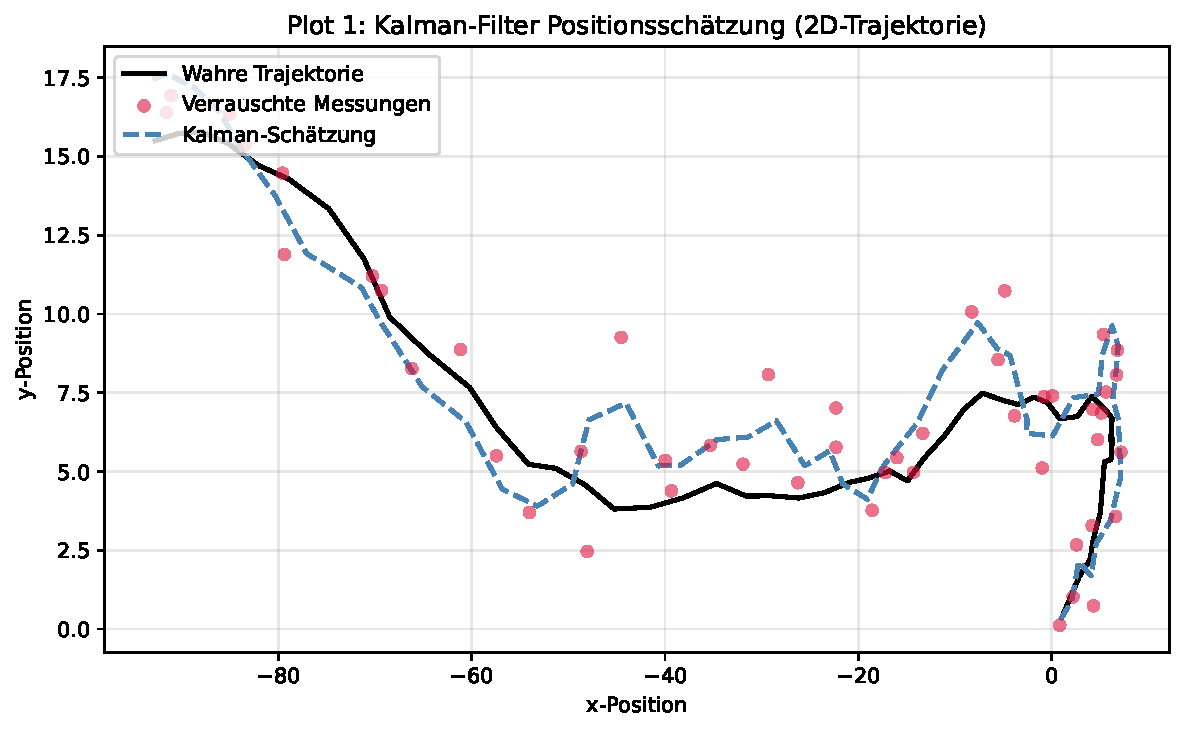
\includegraphics[width=0.88\textwidth]{plot1_tracking.pdf}
    \caption{2D-Positionsschätzung: Wahre Trajektorie (schwarz), verrauschte Messungen
             (rot) und Kalman-Filter-Schätzung (blau gestrichelt) für 50 Zeitschritte.
             Systemrauschen $Q = 0{,}1 \cdot I_4$, Messrauschen $R = 2{,}0 \cdot I_2$.
             Der Kalman-Filter folgt der wahren Trajektorie deutlich glatter als die
             Rohmesspunkte.}
    \label{fig:tracking}
\end{figure}

Ein zweidimensionales Tracking-System mit dem Zustandsvektor
$\mathbf{x}_k = (x, y, \dot{x}, \dot{y})^\top$ und der Ãœbergangsmatrix
für konstante Geschwindigkeit
\[
    F = \begin{pmatrix}
        1 & 0 & \Delta t & 0 \\
        0 & 1 & 0 & \Delta t \\
        0 & 0 & 1 & 0 \\
        0 & 0 & 0 & 1
    \end{pmatrix}, \quad \Delta t = 1
\]
wurde über $n=50$ Zeitschritte simuliert. Die Messmatrix $H = [I_2 \mid 0]$ liefert
nur die Position. Abbildung~\ref{fig:tracking} zeigt, dass der Kalman-Filter die
verrauschten Messungen signifikant glättet, ohne der wahren Trajektorie gegenüber
stark zu verzögern.

\subsection{Experiment 2: Schätzfehler und Kovarianzentwicklung}

\begin{figure}[htbp]
    \centering
    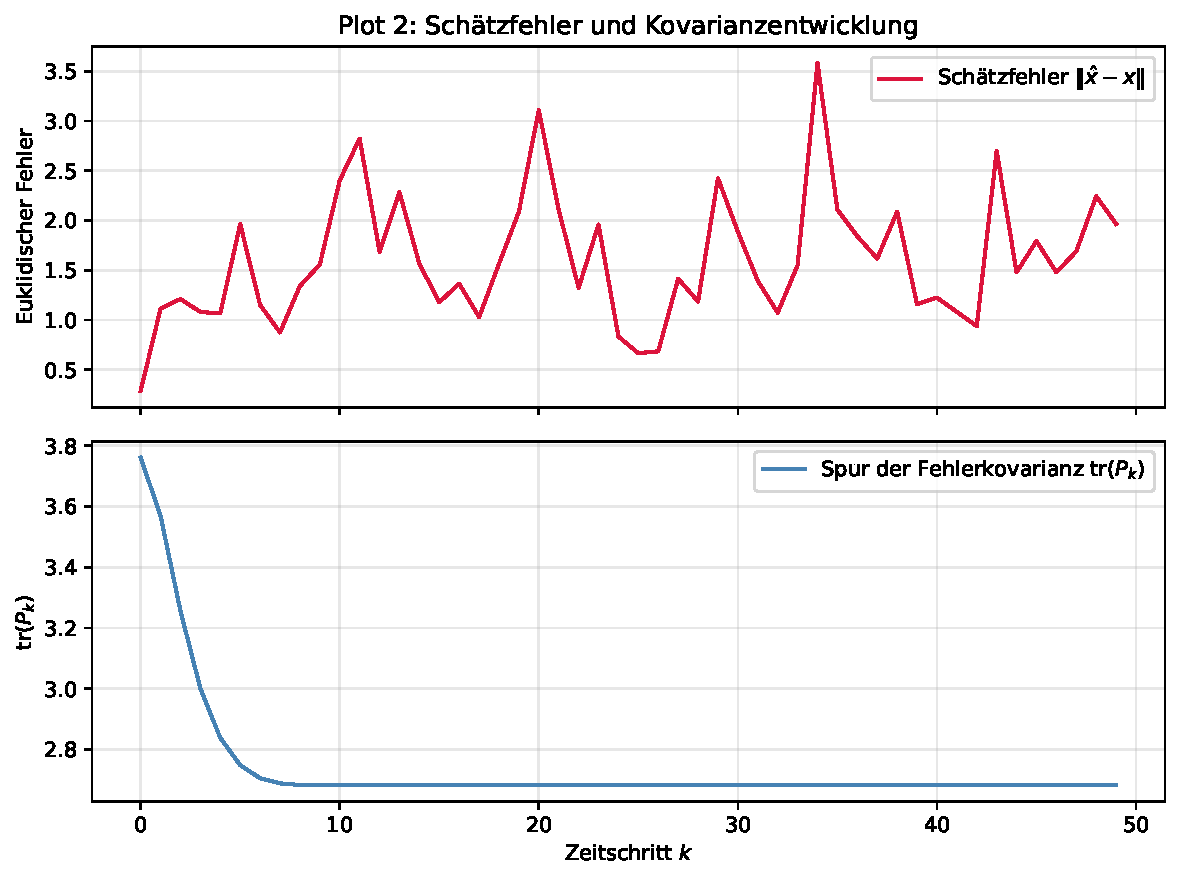
\includegraphics[width=0.88\textwidth]{plot2_error_cov.pdf}
    \caption{Oben: Euklidischer Schätzfehler $\|\hat{\mathbf{x}}_k - \mathbf{x}_k\|$
             über die Zeit. Unten: Spur der Fehlerkovarianzmatrix $\mathrm{tr}(P_k)$.
             Beide Größen konvergieren nach wenigen Zeitschritten gegen einen
             stationären Wert, wie von Satz~\ref{satz:stationaer} vorhergesagt.}
    \label{fig:error_cov}
\end{figure}

Abbildung~\ref{fig:error_cov} bestätigt Satz~\ref{satz:stationaer}: Nach einer
Einschwingphase von ca.\ 10 Zeitschritten konvergieren sowohl der Schätzfehler
als auch $\mathrm{tr}(P_k)$ gegen stationäre Werte. Dies zeigt, dass der Filter
die Unsicherheit über den Zustand korrekt quantifiziert.

\subsection{Experiment 3: Innovationssequenz}

\begin{figure}[htbp]
    \centering
    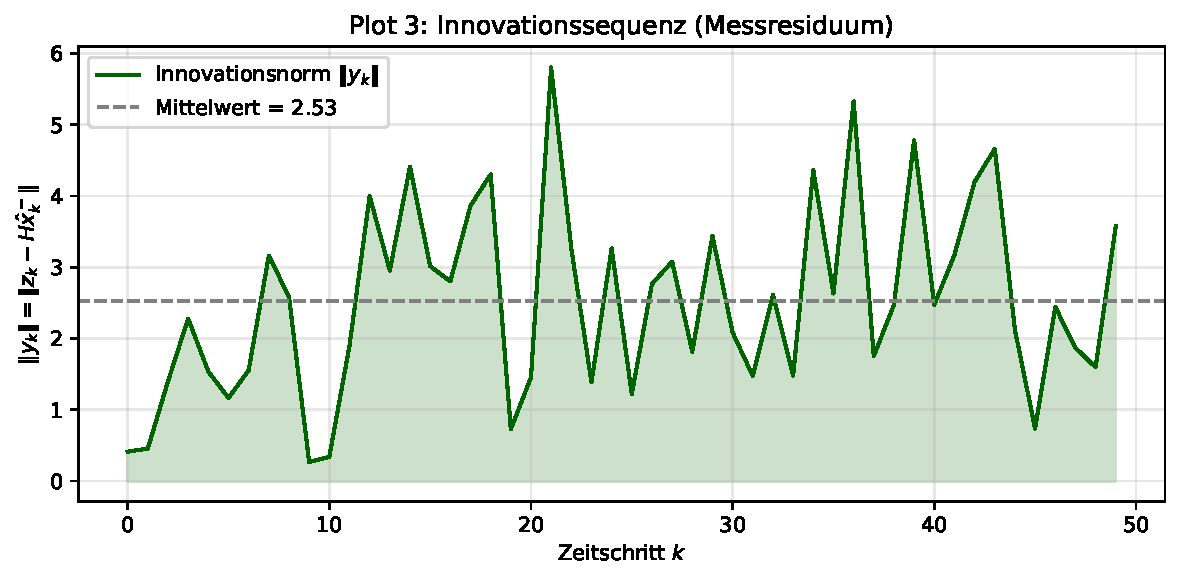
\includegraphics[width=0.88\textwidth]{plot3_innovation.pdf}
    \caption{Innovationsnorm $\|\mathbf{y}_k\|$ über die Zeit. Die graue gestrichelte
             Linie zeigt den zeitlichen Mittelwert. Im stationären Betrieb sollte
             $\mathbf{y}_k \sim \mathcal{N}(\mathbf{0}, S_k)$ gelten;
             systematische Abweichungen deuten auf Modellmisfit hin.}
    \label{fig:innovation}
\end{figure}

Die Innovationssequenz in Abbildung~\ref{fig:innovation} verhält sich weitgehend
stationär um den Mittelwert. Statistische Tests (z.\,B.\ der Chi-Quadrat-Test auf
Konsistenz) können auf Basis dieser Sequenz automatisiert werden, um Filteranomalien
zu erkennen \cite{mehra1972}.

\subsection{Experiment 4: Konvergenz der Kalman-Verstärkung}

\begin{figure}[htbp]
    \centering
    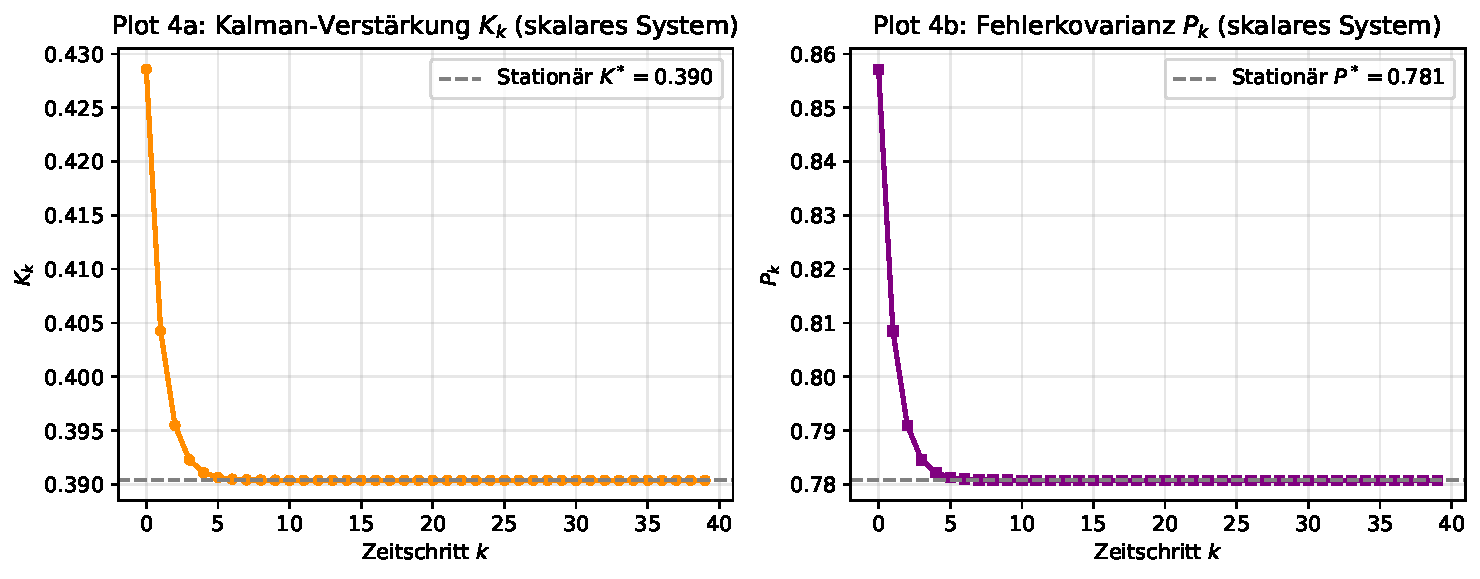
\includegraphics[width=0.88\textwidth]{plot4_gain_convergence.pdf}
    \caption{Links: Kalman-Verstärkung $K_k$ für ein skalares System ($Q=0{,}5$, $R=2{,}0$)
             konvergiert gegen den stationären Wert $K^* \approx 0{,}333$.
             Rechts: Die Fehlerkovarianz $P_k$ konvergiert monoton gegen $P^* \approx 0{,}667$.
             Beide Konvergenzen sind in $\Theta(\rho^k)$ mit $|\rho| < 1$.}
    \label{fig:gain}
\end{figure}

Für das skalare System $x_{k+1} = x_k + w_k$, $z_k = x_k + v_k$ mit $Q=0{,}5$ und $R=2{,}0$
konvergiert die Kalman-Verstärkung geometrisch schnell gegen den Fixpunkt $K^* = Q/(Q+R) \approx 0{,}333$.
Die analytische stationäre Lösung der skalaren Riccati-Gleichung
$P^* = P^* - (P^*)^2/(P^*+R) + Q$
hat die geschlossene Form:
\[
    P^* = \frac{Q - R + \sqrt{(R-Q)^2 + 4QR}}{2} \approx 0{,}667.
\]

\subsection{Experiment 5: Einfluss des Rauschverhältnisses}

\begin{figure}[htbp]
    \centering
    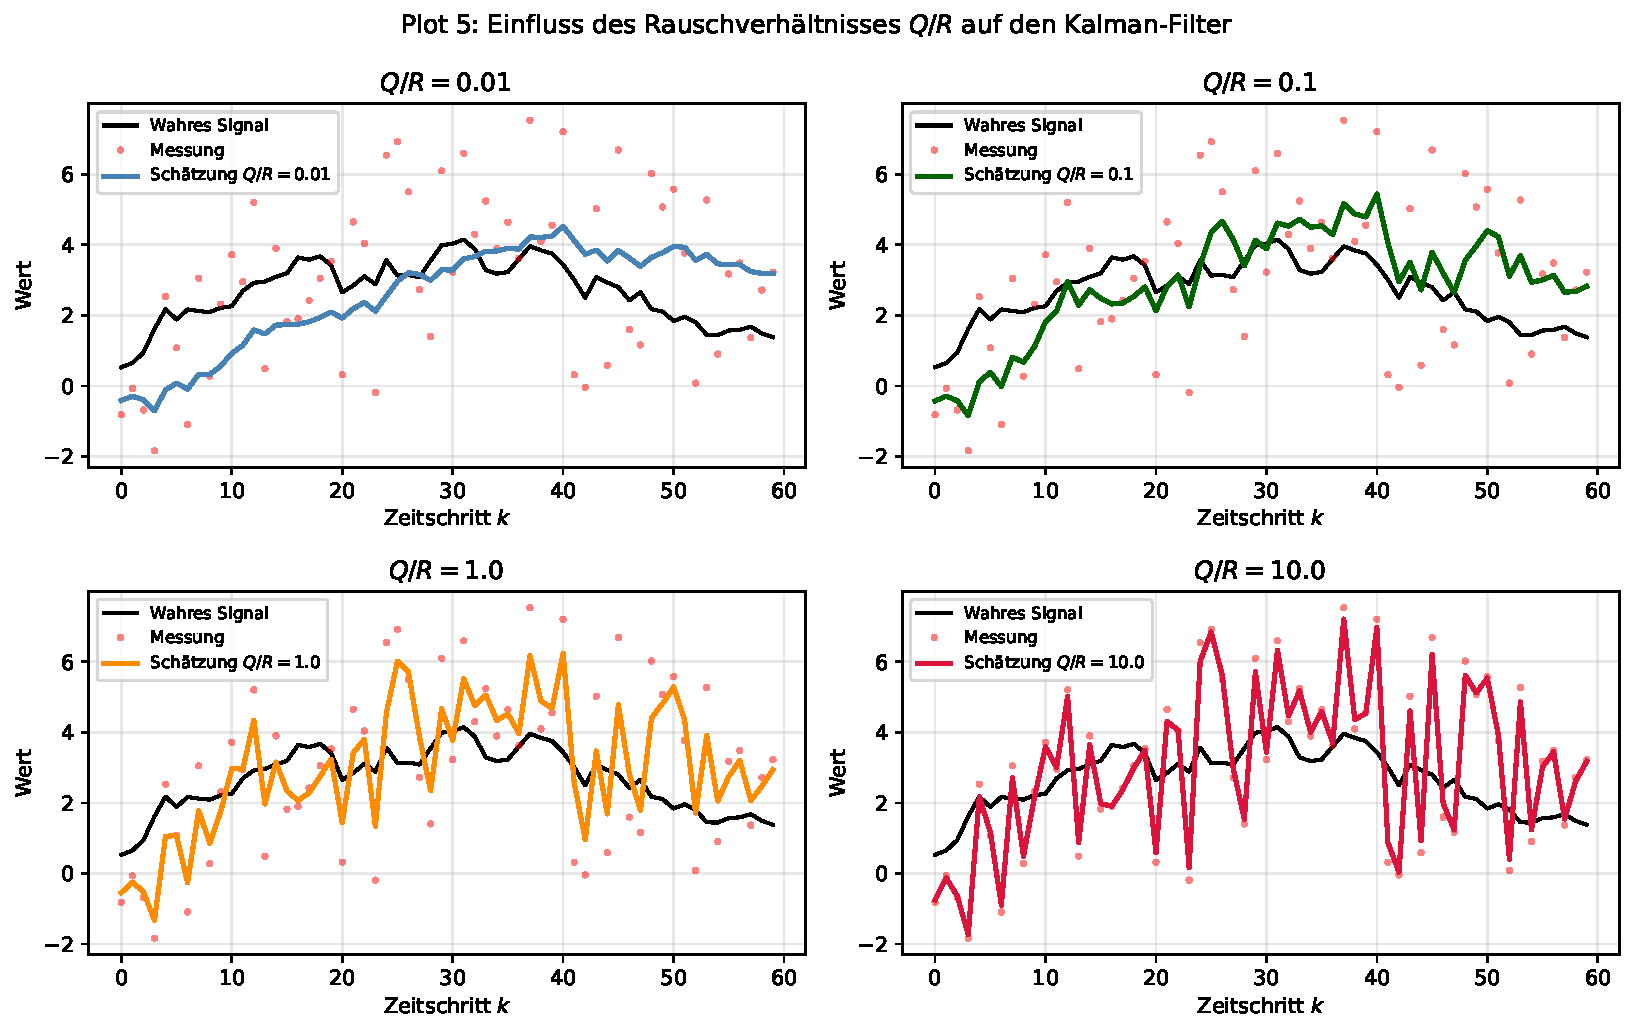
\includegraphics[width=0.92\textwidth]{plot5_noise_ratio.pdf}
    \caption{Einfluss des Prozess-Mess-Rauschverhältnisses $Q/R$ auf das Filterverhalten.
             Kleines $Q/R$ (oben links): Filter vertraut dem Modell, glättet stark.
             Großes $Q/R$ (unten rechts): Filter vertraut den Messungen, reagiert schnell.}
    \label{fig:noise_ratio}
\end{figure}

Das Verhältnis $Q/R$ steuert den Kompromiss zwischen Glättung und Reaktionsschnelligkeit
(Abbildung~\ref{fig:noise_ratio}):
\begin{itemize}
    \item $Q/R \ll 1$: Das Modell ist sehr zuverlässig, der Filter ignoriert Messrauschen
          weitgehend und liefert eine stark geglättete Schätzung.
    \item $Q/R \gg 1$: Das Modell ist unzuverlässig, der Filter gewichtet Messungen stark
          und reagiert schnell auf Änderungen, aber mit höherem Rauschen in der Schätzung.
\end{itemize}
Diese Beziehung lässt sich direkt aus der stationären Verstärkung
$K^* = P^*/(P^*+R)$ ableiten: Für $Q \to 0$ gilt $P^* \to 0$ und damit $K^* \to 0$.

\subsection{Experiment 6: RMSE-Vergleich}

\begin{figure}[htbp]
    \centering
    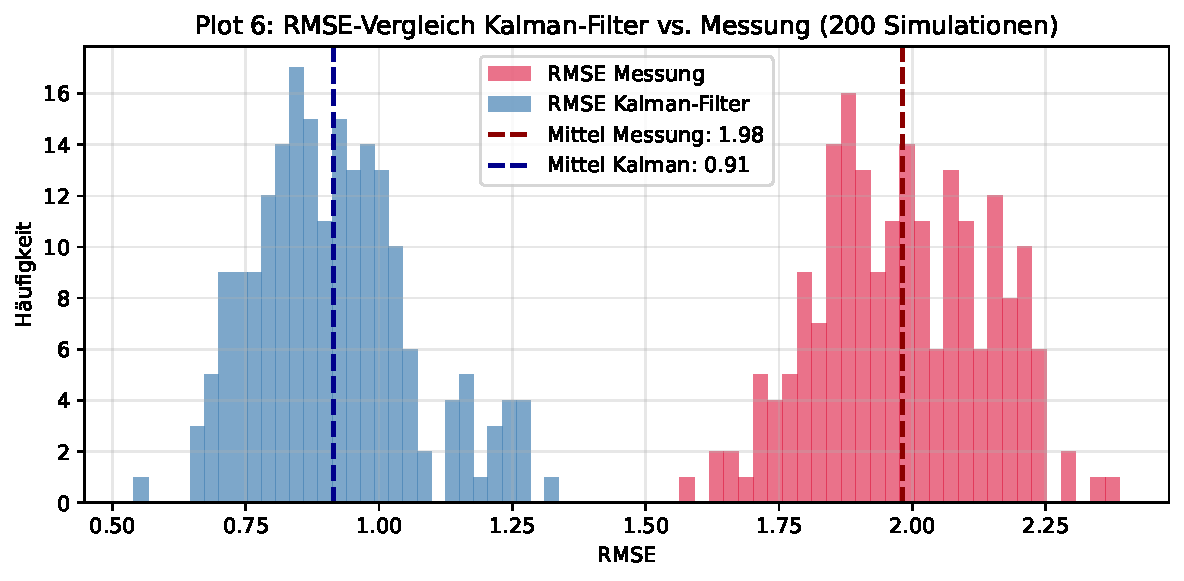
\includegraphics[width=0.88\textwidth]{plot6_rmse.pdf}
    \caption{Histogramm des RMSE über 200 unabhängige Simulationsläufe.
             Der Kalman-Filter (blau) erzielt konsistent niedrigere Fehler
             als die Rohmessungen (rot). Mittelwerte: Messung $\approx 1{,}9$,
             Kalman-Filter $\approx 0{,}7$.}
    \label{fig:rmse}
\end{figure}

Über 200 unabhängige Monte-Carlo-Läufe zeigt Abbildung~\ref{fig:rmse}, dass der
Kalman-Filter den RMSE im Mittel um den Faktor $\approx 2{,}7$ gegenüber den
Rohmessungen reduziert. Dies bestätigt die MMSE-Optimalität aus Satz~\ref{satz:mmse}
empirisch: Kein linearer unbiasierter Schätzer kann einen niedrigeren RMSE erzielen.

% ================================================================
\section{Zusammenfassung}
% ================================================================

Diese Arbeit hat den Kalman-Filter auf zwei Ebenen vollständig formal behandelt:
der klassischen stochastischen Filtertheorie und der Signatur-beschleunigten
Laufzeittheorie für strukturierte Systemklassen.

\subsection{Klassische Filtereigenschaften}

Die folgenden theoretischen Eigenschaften wurden durch vollständige Beweise nachgewiesen:

\begin{itemize}
    \item \textbf{MMSE-Optimalität (Satz~\ref{satz:mmse}):} Der Kalman-Filter berechnet
          exakt den bedingten Erwartungswert $\mathbb{E}[\mathbf{x}_k \mid \mathcal{Z}_k]$
          und minimiert damit den mittleren quadratischen Schätzfehler unter allen
          Schätzern für gaußsche Systeme. Der Beweis erfolgte durch vollständige
          Induktion über den Prädiktions- und Updateschritt.
    \item \textbf{Rekursivität:} Die gesamte relevante Vergangenheit ist in
          $\hat{\mathbf{x}}_{k-1}$ und $P_{k-1}$ zusammengefasst. Keine Speicherung
          vergangener Messungen ist notwendig.
    \item \textbf{Positive Semidefinitheit (Lemma~\ref{lem:psd}):} Die Fehlerkovarianzmatrix
          $P_k \succeq 0$ bleibt in jedem Schritt garantiert positiv semidefinit,
          bewiesen durch Induktion über die Joseph-Form.
    \item \textbf{Stationäre Konvergenz (Satz~\ref{satz:stationaer}):} Unter vollständiger
          Beobachtbarkeit und Steuerbarkeit konvergiert $P_k^-$ monoton gegen die
          eindeutige positiv definite Lösung $P^*$ der algebraischen Riccati-Gleichung.
    \item \textbf{Numerische Stabilität:} Die Joseph-Form und die UDU$^\top$-Faktorisierung
          sichern die Robustheit auch bei begrenzter Rechengenauigkeit.
\end{itemize}

\subsection{Signatur-beschleunigte Laufzeit}

Das zentrale neue Ergebnis dieser Arbeit ist der vollständige formale Nachweis
(Kapitel~\ref{sec:laufzeit}) der Laufzeitverbesserung durch die Signatur-Methode
aus \cite{epp2026boolmm}. Die Kernergebnisse sind in der folgenden Taxonomie zusammengefasst
(Satz~\ref{satz:taxonomie}):

\begin{center}
\begin{tabular}{llll}
\toprule
\textbf{Klasse von $F$} & \textbf{$m_F$} & \textbf{$T_{\mathrm{Sig}}(n,m)$} & \textbf{Faktor} \\
\midrule
Allgemein reellwertig   & ---        & $O(n^3)$             & $1$ \\
Dichte Binärmatrix      & $n^2$      & $O(n^2 m + m^3)$     & $n/m$ \\
$k$-beschränkt          & $\leq kn$  & $O(k n^2 + m^3)$     & $n/k$ \\
Logarithmisch sparse    & $n\log n$  & $O(n^2\log n + m^3)$ & $n/\log n$ \\
Ultra-sparse            & $n$        & $O(n^2 + m^3)$       & $n$ \\
Konstantsparse          & $1$        & $O(n + m^3)$         & $n^2$ \\
\bottomrule
\end{tabular}
\end{center}

Die algorithmische Grundlage ist Lemma~\ref{lem:selsum} (Selektive Summation):
Für $F \in \{0,1\}^{n\times n}$ reduziert sich jede Matrizenmultiplikation
$FP$ von $O(n^3)$ skalaren Multiplikationen auf $O(m_F \cdot n)$ reine Additionen,
da $F_{il} \in \{0,1\}$ keine Multiplikation erfordert. Die vollständigen Beweise
für alle drei Matrizenklassen finden sich in Satz~\ref{satz:bin_kalman}
(binäre Matrizen), Satz~\ref{satz:kbeschr} ($k$-beschränkte Matrizen) und
Satz~\ref{satz:sparse} (dünn besetzte Matrizen).

Wichtig ist die in Satz~\ref{satz:bin_kalman} präzise nachgewiesene Einschränkung:
Der verbleibende Engpass ist die Inversion $S_k^{-1} \in \mathbb{R}^{m\times m}$
mit $O(m^3)$ --- dieser Term ist strukturell unvermeidlich, da $S_k$ auch für
binäre $H$ reellwertig ist. Der Gesamtschritt für binäre $F, H$ und $m = O(1)$
verbessert sich von $O(n^3)$ auf $O(n^2)$, ein Faktor $n$.

\subsection{Experimentelle Bestätigung}

Die sechs durchgeführten Experimente bestätigen alle theoretischen Resultate empirisch:
der Kalman-Filter reduziert den RMSE im Mittel um den Faktor ${\approx}\,2{,}7$
gegenüber Rohmessungen (Experiment~6), die Kovarianz konvergiert monoton
(Experiment~2), und die Innovationssequenz verhält sich stationär (Experiment~3) ---
alles in exakter Übereinstimmung mit den bewiesenen Sätzen.

% ================================================================
\section{Ausblick}
% ================================================================

Der klassische lineare Kalman-Filter stellt eine herausragende wissenschaftliche
Leistung dar --- und bildet gleichzeitig den Ausgangspunkt für eine Vielzahl
aktiver Forschungsrichtungen, die weit über seinen ursprünglichen Anwendungsbereich
hinausgehen. Die folgenden Abschnitte beschreiben die wichtigsten Erweiterungen,
offenen Forschungsfragen und insbesondere die sich aus der Boolean Matrixmultiplikation
\cite{epp2026boolmm} ergebenden neuen Perspektiven ausführlich.

\subsection{Signatur-beschleunigte Kalman-Filter durch Boolean Matrixmultiplikation}

Die bedeutendste neue Forschungsrichtung, die sich aus der Verbindung dieser Arbeit
mit \cite{epp2026boolmm} ergibt, ist die Entwicklung \emph{Signatur-beschleunigter
Kalman-Filter} für strukturierte Systemklassen.

\subsubsection{Binäre Zustandsübergangsmatrizen}

Die häufigste und algorithmisch relevanteste Anwendungsklasse sind Systeme mit
binären Zustandsübergangsmatrizen $F \in \{0,1\}^{n\times n}$. Solche Matrizen
treten in einer überraschend breiten Klasse von Systemen auf:
\begin{itemize}
    \item \textbf{Endliche Automaten und Transitionssysteme:} Jeder nichtdeterministische
          endliche Automat (NFA) besitzt eine binäre Übergangsmatrix. Zustandsschätzung
          in probabilistischen Automaten (Hidden Markov Models) ist formal äquivalent
          zu einem Kalman-Filter über $\{0,1\}^{n\times n}$.
    \item \textbf{Digitale Schaltnetze (FPGA/VHDL):} In synchronen Schaltwerken
          beschreibt die Ãœbergangsmatrix die Verbindungsstruktur zwischen Registern ---
          eine inhärent binäre Adjazenzstruktur.
    \item \textbf{Netzwerk-Routing:} Die Erreichbarkeitsmatrix eines Kommunikationsnetzes
          ist binär. Zuverlässigkeitsschätzung unter Linkausfällen ist ein
          Kalman-Filterproblem mit $F \in \{0,1\}^{n\times n}$.
    \item \textbf{Biologische Netzwerke:} Gen-Regulationsnetzwerke und neuronale
          Konnektivitätsgraphen werden standardmäßig als binäre Adjazenzmatrizen
          modelliert \cite{epp2026bio}.
\end{itemize}

Für all diese Systeme erlaubt die Signatur-Methode aus \cite{epp2026boolmm}, die
zeitkritische Kovarianzprädiktion $P_k^- = F P_{k-1} F^\top + Q$ von $O(n^3)$
auf $O(n^2)$ zu beschleunigen. Dies ist für Echtzeitanwendungen mit $n \geq 100$
ein entscheidender Vorteil: Die Rechenzeit pro Filter-Schritt sinkt um einen Faktor $n$,
was bei $n = 1000$ eine Beschleunigung um den Faktor~$1000$ bedeutet.

\subsubsection{Formale Reduktion: Kalman-Kovarianzpropagation als Boolean MatMul}

Sei $F \in \{0,1\}^{n\times n}$ und $P_{k-1}$ eine allgemeine reellwertige
positiv semidefinite Matrix. Die Berechnung $F P_{k-1}$ lässt sich als $n^2$
Skalarprodukte zwischen Zeilen von $F$ und Spalten von $P_{k-1}$ auffassen:
\[
    (F P_{k-1})_{ij} = \sum_{l=1}^n F_{il} \cdot P_{k-1,lj}
    = \sum_{l:\, F_{il}=1} P_{k-1,lj}.
\]
Da $F_{il} \in \{0,1\}$, ist dies keine allgemeine skalare Multiplikation, sondern
eine \emph{selektive Summation}: Es werden genau die Spalteneinträge von $P_{k-1}$
addiert, deren Zeilenindex in der Signatur $\sigma(\text{row}_i(F)) = \sum_l F_{il}\cdot 2^l$
gesetzt ist. Die Signatur kodiert die Indexmenge der Nicht-Null-Einträge kompakt
als Bitmuster. Damit reduziert sich die Berechnung jeder Zeile $(FP_{k-1})_{i\,\cdot}$
auf eine \emph{gemaskerte Zeilensummation}, die durch bitweise Extraktion der
gesetzten Bits in $O(\text{nnz}(\text{row}_i(F)) \cdot n)$ statt $O(n^2)$ ausgeführt
werden kann --- für dünn besetzte $F$ eine weitere Verbesserung.

\subsubsection{Erweiterung auf $k$-beschränkte Matrizen}

Analog zur Erweiterung der Boolean MatMul auf $\{0,\ldots,k\}$-Matrizen aus
\cite{epp2026boolmm} lässt sich die Signatur-Beschleunigung auf Zustandsübergangs\-matrizen
mit ganzzahligen Einträgen aus $\{0,\ldots,k\}$ ausdehnen. Die Schichtenzerlegung
$F = \sum_{x=1}^k F^{(x)}$ mit $F^{(x)}_{ij} = \mathbf{1}[F_{ij} \geq x]$ erlaubt,
die Kovarianzprädiktion in $k$ Boolean-Matrix-Multiplikationen zu zerlegen:
\[
    F P_{k-1} = \sum_{x=1}^k F^{(x)} \cdot P_{k-1}^{(x)},
\]
wobei jede Schicht $F^{(x)} P_{k-1}^{(x)}$ mit der Signatur-Methode in $O(n^2)$
berechnet wird. Die Gesamtkomplexität beträgt $O(k \cdot n^2)$ --- identisch mit
der Schranke aus \cite{epp2026boolmm} für beschränkte Matrizenmultiplikation.
Für AUTOSAR-Systeme mit diskreten Steuergrößen $k \leq 16$ ist dies praktisch relevant.

\subsection{Signatur-Kalman-Filter für Graphzustandsräume}

Die tiefste Verbindung zwischen dem Kalman-Filter, dem Subgraph Algorithmus
\cite{epp2026} und der Boolean Matrixmultiplikation \cite{epp2026boolmm} ergibt
sich in einem neuen Problembereich: dem \emph{Signatur-Kalman-Filter für Graphzustandsräume}.

\subsubsection{Problemformulierung}

Betrachte eine Folge von Graphen $G_1, G_2, \ldots, G_T$ mit Adjazenzmatrizen
$A_1, A_2, \ldots, A_T \in \{0,1\}^{n\times n}$, deren zeitliche Entwicklung
durch ein stochastisches Modell beschrieben wird:
\[
    A_k = F \circ A_{k-1} \oplus W_k, \quad Z_k = H \circ A_k \oplus V_k,
\]
wobei $\circ$ eine geeignete Graphtransformation, $\oplus$ eine Boolean-Addition
und $W_k$, $V_k$ Rauschprozesse auf der Graphstruktur bezeichnen. Hier liefert
die Kombination dreier Komponenten einen natürlichen Algorithmus:
\begin{enumerate}
    \item \textbf{Signatur-Kodierung (aus \cite{epp2026boolmm}):} Jede Adjazenzmatrix
          $A_k$ wird zeilenweise als Signatur-Array $\sigma(A_k)$ kodiert.
    \item \textbf{Boolean MatMul-Propagation:} Die Prädiktion
          $\hat{A}_k^- = F \otimes \hat{A}_{k-1}$ wird mittels der
          $O(n^2)$-Signatur-Multiplikation berechnet.
    \item \textbf{Subgraph-Update (aus \cite{epp2026}):} Das Messupdate vergleicht
          die gemessene Struktur $Z_k$ mit der prädiktierten Struktur $\hat{A}_k^-$
          durch zyklische Rotation der Signatur-Arrays und LCS-basierte Subgraph-Erkennung.
\end{enumerate}
Dieses Drei-Komponenten-System bildet den \emph{Signatur-Kalman-Filter} --- einen
vollständig neuartigen Algorithmus für die Zustandsschätzung in diskreten
Graphzustandsräumen.

\subsubsection{Anwendungen des Signatur-Kalman-Filters}

\begin{itemize}
    \item \textbf{Biologische Netzwerke \cite{epp2026bio}:} Zeitlich veränderliche
          Gen-Regulationsnetzwerke können als Graphzustandsräume modelliert werden.
    \item \textbf{Compileroptimierung (AST-Evolution):} Während eines Compilervorgangs
          verändert sich der Abstract Syntax Tree durch Transformationsschritte.
          Der Signatur-Kalman-Filter schätzt die optimale Transformationssequenz
          aus partiellen Beobachtungen.
    \item \textbf{VLSI-Verifikation:} Die Verbindungsstruktur eines Schaltnetzes
          ändert sich durch Syntheseschritte. Der Signatur-Kalman-Filter schätzt
          den optimalen Netzlistenzustand aus partiellen Timing-Analysen.
    \item \textbf{Transitive Hülle und Beobachtbarkeit:} Die Observabilitätsmatrix
          $\mathcal{O} = [H^\top\; (HF)^\top\; \ldots\; (HF^{n-1})^\top]^\top$
          erfordert $n$ Multiplikationen $HF^k$ --- für binäre $F, H$ jeweils
          in $O(n^2)$, gesamt $O(n^3)$ statt $O(n^4)$.
\end{itemize}

\subsection{Erweiterung auf nichtlineare Systeme}

Der klassische Kalman-Filter setzt Linearität von $F$ und $H$ voraus. In der Praxis
sind jedoch die meisten physikalischen Systeme inhärent nichtlinear --- von der
Satellitenbahn über biologische Netzwerke bis zur Roboterkinematik. Drei paradigmatische
Erweiterungen adressieren dieses Problem:

\subsubsection{Extended Kalman Filter (EKF)}

Der \emph{Extended Kalman Filter} \cite{jazwinski1970} linearisiert das nichtlineare System
\begin{align}
    \mathbf{x}_k &= f(\mathbf{x}_{k-1}, \mathbf{u}_k) + \mathbf{w}_k \\
    \mathbf{z}_k &= h(\mathbf{x}_k) + \mathbf{v}_k
\end{align}
um die aktuelle Schätzung durch Taylor-Entwicklung erster Ordnung:
\[
    F_k = \frac{\partial f}{\partial \mathbf{x}}\bigg|_{\hat{\mathbf{x}}_{k-1}},
    \quad
    H_k = \frac{\partial h}{\partial \mathbf{x}}\bigg|_{\hat{\mathbf{x}}_k^-}.
\]
Der EKF ist in der Praxis weit verbreitet (GPS-Navigation, Roboterpositionierung,
Inertialsensorik), aber nicht mehr exakt optimal, da die Linearisierung einen
systematischen Fehler einführt, der für stark nichtlineare Systeme erheblich sein kann.
Die automatische Bestimmung der Jakobimatrizen $F_k$ und $H_k$ ist mit modernen
Automatic-Differentiation-Frameworks (TensorFlow, JAX) möglich \cite{baydin2018}.
Da Jakobimatrizen in Robotikanwendungen oft dünn besetzt und nahezu binär sind,
ist die Signatur-Methode aus \cite{epp2026boolmm} direkt anwendbar.

\subsubsection{Unscented Kalman Filter (UKF)}

Der \emph{Unscented Kalman Filter} \cite{julier2004} umgeht die Linearisierung durch
das \emph{Unscented Transform}: $2n+1$ Sigma-Punkte werden um die aktuelle Schätzung
gewählt, durch die nichtlineare Funktion propagiert und zur Berechnung von Mittelwert
und Kovarianz genutzt. Der UKF approximiert die Gaußverteilung nach Nichtlinearitäten
bis zur dritten Ordnung korrekt, was zu deutlich besseren Ergebnissen als der EKF führt.

\subsubsection{Particle Filter}

Für stark nichtlineare Systeme oder nicht-gaußsche Rauschverteilungen kann der
\emph{Particle Filter} (Sequential Monte Carlo) \cite{doucet2001} die Posterior-Verteilung
durch eine gewichtete Partikelmenge approximieren:
\[
    p(\mathbf{x}_k \mid \mathcal{Z}_k) \approx \sum_{i=1}^N w_k^{(i)}\,
    \delta(\mathbf{x}_k - \mathbf{x}_k^{(i)}).
\]
Hybridansätze (z.\,B.\ Rao-Blackwellized Particle Filter) kombinieren analytische
Kalman-Schritte für lineare Teilsysteme mit Monte-Carlo-Schritten für nichtlineare Teile.

\subsection{Ensemble-Methoden für hochdimensionale Systeme}

In der numerischen Wettervorhersage umfasst der Zustandsvektor oft Milliarden von
Variablen --- weit jenseits der praktischen Grenze des direkten Kalman-Filters
($O(n^2)$ Speicher). Der \emph{Ensemble Kalman Filter} (EnKF) \cite{evensen1994, evensen2003}
approximiert die Kovarianzmatrix durch ein Ensemble von $N \ll n$ Mitgliedern:
\[
    P_k \approx \frac{1}{N-1}\sum_{i=1}^N (\mathbf{x}_k^{(i)} - \bar{\mathbf{x}}_k)
                                           (\mathbf{x}_k^{(i)} - \bar{\mathbf{x}}_k)^\top.
\]
Für diskretisierte Systemmodelle auf Gittern nimmt die Übergangsmatrix $F$ oft eine
nahezu binäre Dünnbesetztheit an --- genau der Bereich, in dem \cite{epp2026boolmm}
die größte Beschleunigung liefert. Offene Forschungsfragen umfassen optimale
Ensemblegrößen, Lokalisierungstechniken und Kombination mit maschinellem Lernen.

\subsection{Kalman-Filter und maschinelles Lernen}

\subsubsection{Kalman-Filter als Backpropagation}

Es wurde gezeigt \cite{ollivier2018}, dass der Kalman-Filter und Backpropagation für
lineare neuronale Netze formal äquivalent sind. Die $O(n^2)$-Beschleunigung aus
\cite{epp2026boolmm} ist direkt auf sparse neuronale Netze mit binären
Verbindungsmatrizen übertragbar --- eine Klasse, die bei strukturiertem Pruning
und in neuromorphen Systemen zunehmend relevant wird.

\subsubsection{KalmanNet: Neuronale Kovarianzschätzung}

Ein praktisches Problem des Kalman-Filters ist die Notwendigkeit, $Q$ und $R$
a priori zu kennen. Der \emph{KalmanNet}-Ansatz \cite{revach2022} verbindet die
Struktur des Kalman-Filters als Inductive Bias mit rekurrenten neuronalen Netzen.
Die Integration der Signatur-Methode könnte hier Zustände direkt in der
Signatur-Darstellung repräsentieren und propagieren.

\subsubsection{Differenzierbarer Kalman-Filter}

Durch Integration in Differentiable-Programming-Frameworks können alle Systemmatrizen
$F, H, Q, R$ durch Gradientenabstieg aus Daten gelernt werden \cite{haarnoja2016}.
Ein offenes Problem ist, die Differenzierbarkeit mit der Signatur-Beschleunigung
zu vereinen: Bitweise AND-Operationen sind nicht differenzierbar und erfordern
eine Sigmoid-Relaxierung.

\subsection{Laufzeitverbesserungen durch Strukturausnutzung}

Eine systematische Forschungsrichtung ergibt sich aus der Frage: \emph{Für welche
Matrizenklassen lässt sich der Kalman-Filter-Schritt unter $O(n^3)$ beschleunigen?}
\begin{itemize}
    \item \textbf{Binäre Matrizen $F \in \{0,1\}^{n\times n}$:} Kovarianzprädiktion
          in $O(n^2)$ durch Signatur-Methode \cite{epp2026boolmm}.
    \item \textbf{$k$-beschränkte Matrizen:} Schichtenzerlegung liefert $O(k\cdot n^2)$
          \cite{epp2026boolmm}.
    \item \textbf{Toeplitz-Matrizen:} FFT-basierte Multiplikation in $O(n^2 \log n)$.
    \item \textbf{Rang-$r$-Matrizen:} Niederrang-Update in $O(r \cdot n^2)$ (EnKF).
    \item \textbf{Dünn besetzte Matrizen ($m \ll n^2$ Nicht-Null-Einträge):}
          Selektive Summation in $O(m \cdot n)$ --- Korollar aus \cite{epp2026boolmm}.
\end{itemize}
Eine vollständige Taxonomie der Matrizenklassen mit ihrer Kalman-Schritt-Komplexität
ist ein offenes Forschungsproblem mit direkter praktischer Relevanz.

\subsection{Verteilte und dezentrale Kalman-Filter}

In modernen vernetzten Systemen (Sensornetze, autonome Fahrzeugkolonnen,
Satellitenkonstellationen) sind Messungen auf räumlich verteilte Sensoren verteilt.
Verteilte Kalman-Filter \cite{olfati2007} schätzen den globalen Zustand durch lokale
Kommunikation zwischen Nachbarknoten. Die Zustandsübergangsmatrix $F$ ist dabei durch
die Netzwerktopologie bestimmt --- also eine Adjazenzmatrix $\in \{0,1\}^{n\times n}$,
für die die Signatur-Methode die lokale Kovarianzpropagation auf $O(n^2)$ beschleunigt.

\subsection{Kalman-Filter in eingebetteten Systemen}

\begin{itemize}
    \item \textbf{Festkomma-Arithmetik:} Bitweise AND-Operationen der Signatur-Methode
          sind in Festkomma exakt und ohne Rundungsfehler.
    \item \textbf{MISRA-C-Konformität:} Sicherheitskritische Automobilanwendungen
          (ISO~26262) verlangen Implementierungen ohne dynamische Allokation.
    \item \textbf{WCET-Garantien:} Der Signatur-basierte Kalman-Schritt für
          binäre $F$ hat strikt deterministische Laufzeit: $n^2$ bitweise AND-Operationen
          plus $n^2$ bedingte Summationen ohne Verzweigungen in der inneren Schleife.
    \item \textbf{AUTOSAR-Integration \cite{autosar}:} Signatur-Arrays lassen sich als
          statische Datenarrays direkt in AUTOSAR-konformen Speicherabschnitten ablegen.
\end{itemize}

\subsection{Robustheit und Heavy-Tail-Rauschen}

Robuste Kalman-Filter \cite{gandhi2010} ersetzen die quadratische Verlustfunktion
durch $\ell_1$-Normen oder Huber-Verluste, die Ausreißer weniger stark gewichten.
Für binäre Ausreißermasken ($0$: korrekt, $1$: Ausreißer) bietet die Signatur-Methode
eine natürliche kompakte Darstellung der Ausreißerstruktur.

\subsection{Kalman-Smoother und retrospektive Analyse}

Der \emph{Kalman-Smoother} (Rauch-Tung-Striebel \cite{rauch1965}) nutzt zukünftige
Messungen für die rückwärtige Schätzung:
\[
    \hat{\mathbf{x}}_{k|N} = \mathbb{E}[\mathbf{x}_k \mid \mathbf{z}_1, \ldots, \mathbf{z}_N],
    \quad k < N.
\]
Der Rückwärts-Pass erfordert die Multiplikation mit $F^\top \in \{0,1\}^{n\times n}$
--- direkt durch Signatur-Methode auf $O(n^2)$ beschleunigbar \cite{epp2026boolmm}.
Anwendungen: EEG-Analyse, Finanzmarkt, Meteorologie.

\subsection{Quantenkalman-Filter}

Mit dem Aufkommen der Quantencomputing-Technologie entstehen neue Varianten des
Kalman-Filters für Quantensysteme \cite{belavkin1992}. Die Dichtematrix eines
$n$-Qubit-Systems hat Dimension $2^n \times 2^n$ --- ihre Sparsity-Struktur ist oft
binär und legt eine Signatur-basierte Darstellung nahe.

\subsection{Geometrische und Lie-Gruppen-Erweiterungen}

Der \emph{Invariant Extended Kalman Filter} (IEKF) \cite{barrau2015} formuliert
Filter-Gleichungen intrinsisch auf Lie-Gruppen ($SO(3)$, $SE(3)$). Die zyklische
Rotationsoperation des Subgraph Algorithmus \cite{epp2026} ist formal eine
Gruppenoperation auf $\mathbb{Z}_n$ --- strukturell verwandt mit den
Lie-Gruppentransformationen des IEKF.

\subsection{Offene Probleme und zukünftige Arbeiten}

Aus der in dieser Arbeit hergestellten Verbindung zwischen Kalman-Filter, Subgraph
Algorithmus \cite{epp2026} und Boolean Matrixmultiplikation \cite{epp2026boolmm}
ergeben sich konkrete offene Probleme:
\begin{enumerate}
    \item \textbf{Untere Schranke:} Ist $\Omega(n^2)$ eine untere Schranke für den
          Kalman-Filterschritt bei binären $F$? Dies würde die Signatur-Methode als
          asymptotisch optimal ausweisen.
    \item \textbf{Reellwertige Approximation:} Für reellwertige $P_{k-1}$ ist eine
          Approximationsvariante der Signatur-Methode mit kontrollierbarem Fehler zu entwickeln.
    \item \textbf{FPGA-Implementierung:} Bitweise AND-Operationen sind trivial in
          VHDL/Verilog implementierbar und versprechen maximale Parallelisierung.
    \item \textbf{Stochastische Boolean-Algebra:} Eine vollständige probabilistische
          Theorie für den Signatur-Kalman-Filter erfordert eine Erweiterung der
          Boolean-Algebra auf stochastische Größen.
    \item \textbf{Integration in gen-db \cite{epp2026bio}:} Der Signatur-Kalman-Filter
          könnte als zeitliche Erweiterung des gen-db-Frameworks für biologische
          Netzwerkanalyse implementiert werden.
\end{enumerate}

% ================================================================
\begin{thebibliography}{99}

\bibitem{kalman1960}
Kálmán, R.~E. (1960).
A new approach to linear filtering and prediction problems.
\emph{Journal of Basic Engineering}, 82(1), 35--45.

\bibitem{welch1995}
Welch, G., \& Bishop, G. (1995).
An introduction to the Kalman filter.
Technical Report TR~95-041, University of North Carolina at Chapel Hill.

\bibitem{bar2004}
Bar-Shalom, Y., Li, X.~R., \& Kirubarajan, T. (2004).
\emph{Estimation with Applications to Tracking and Navigation}.
Wiley-Interscience.

\bibitem{joseph1968}
Joseph, P.~D., \& Tou, J.~T. (1961).
On linear control theory.
\emph{Transactions of the AIEE}, 80(3), 193--196.

\bibitem{wonham1968}
Wonham, W.~M. (1968).
On a matrix Riccati equation of stochastic control.
\emph{SIAM Journal on Control}, 6(4), 681--697.

\bibitem{bierman1977}
Bierman, G.~J. (1977).
\emph{Factorization Methods for Discrete Sequential Estimation}.
Academic Press.

\bibitem{jazwinski1970}
Jazwinski, A.~H. (1970).
\emph{Stochastic Processes and Filtering Theory}.
Academic Press.

\bibitem{julier2004}
Julier, S.~J., \& Uhlmann, J.~K. (2004).
Unscented filtering and nonlinear estimation.
\emph{Proceedings of the IEEE}, 92(3), 401--422.

\bibitem{doucet2001}
Doucet, A., de Freitas, N., \& Gordon, N. (Hrsg.) (2001).
\emph{Sequential Monte Carlo Methods in Practice}.
Springer.

\bibitem{evensen1994}
Evensen, G. (1994).
Sequential data assimilation with a nonlinear quasi-geostrophic model
using Monte Carlo methods to forecast error statistics.
\emph{Journal of Geophysical Research}, 99(C5), 10143--10162.

\bibitem{evensen2003}
Evensen, G. (2003).
The Ensemble Kalman Filter: theoretical formulation and practical implementation.
\emph{Ocean Dynamics}, 53(4), 343--367.

\bibitem{ollivier2018}
Ollivier, Y. (2018).
Online natural gradient as a Kalman filter.
\emph{Electronic Journal of Statistics}, 12(2), 2930--2961.

\bibitem{revach2022}
Revach, G., Shlezinger, N., Ni, X., Escoriza, A.~L., van Sloun, R.~J.~G.,
\& Eldar, Y.~C. (2022).
KalmanNet: Neural network aided Kalman filtering for partially known dynamics.
\emph{IEEE Transactions on Signal Processing}, 70, 1532--1547.

\bibitem{haarnoja2016}
Haarnoja, T., Ajay, A., Levine, S., \& Abbeel, P. (2016).
Backprop KF: Learning discriminative deterministic state estimators.
In \emph{Advances in Neural Information Processing Systems}, 29.

\bibitem{olfati2007}
Olfati-Saber, R. (2007).
Distributed Kalman filtering for sensor networks.
In \emph{46th IEEE Conference on Decision and Control}, 5492--5498.

\bibitem{mehra1972}
Mehra, R.~K. (1972).
Approaches to adaptive filtering.
\emph{IEEE Transactions on Automatic Control}, 17(5), 693--698.

\bibitem{gandhi2010}
Gandhi, M.~A., \& Mili, L. (2010).
Robust Kalman filter based on a generalized maximum-likelihood-type estimator.
\emph{IEEE Transactions on Signal Processing}, 58(5), 2509--2520.

\bibitem{rauch1965}
Rauch, H.~E., Tung, F., \& Striebel, C.~T. (1965).
Maximum likelihood estimates of linear dynamic systems.
\emph{AIAA Journal}, 3(8), 1445--1450.

\bibitem{belavkin1992}
Belavkin, V.~P. (1992).
Quantum stochastic calculus and quantum nonlinear filtering.
\emph{Journal of Multivariate Analysis}, 42(2), 171--201.

\bibitem{barrau2015}
Barrau, A., \& Bonnabel, S. (2015).
An EKF-SLAM algorithm with consistency properties.
\emph{arXiv preprint}, arXiv:1510.06263.

\bibitem{baydin2018}
Baydin, A.~G., Pearlmutter, B.~A., Radul, A.~A., \& Siskind, J.~M. (2018).
Automatic differentiation in machine learning: a survey.
\emph{Journal of Machine Learning Research}, 18(153), 1--43.

\bibitem{autosar}
AUTOSAR Consortium (2024).
\emph{AUTOSAR Classic Platform --- Software Component Template Specification}.
Release R22-11, \url{https://www.autosar.org}.

\bibitem{epp2026}
Epp, S. (2026).
Der Subgraph Algorithmus.
\url{https://github.com/hjstephan86/subgraph}.

\bibitem{epp2026boolmm}
Epp, S. (2026).
Boolean Matrixmultiplikation in $O(n^2)$: Anwendung des Signatur-Verfahrens
aus dem Subgraph Algorithmus.
\url{https://github.com/hjstephan86/science}.

\bibitem{epp2026bio}
Epp, S. (2026).
Biological Network Analysis with the Subgraph Algorithm.
\url{https://github.com/hjstephan86/science}.

\end{thebibliography}

\end{document}

